\section{Selected Embedding Visualizations}

Each figure uses seed 4 and the four-thread CPU benchmark profile. When the CPU run is absent but a successful CUDA fastEmbedR run exists, that panel is retained and explicitly marked CUDA. Labels determine point color only and were not used during fitting. A labeled placeholder is retained when the archived run was unavailable, failed, or timed out. FlowRepository and ImageNet contain unmatched fastEmbedR results; those panels demonstrate feasibility only and are excluded from comparative claims.

\begin{figure}[p]
\centering
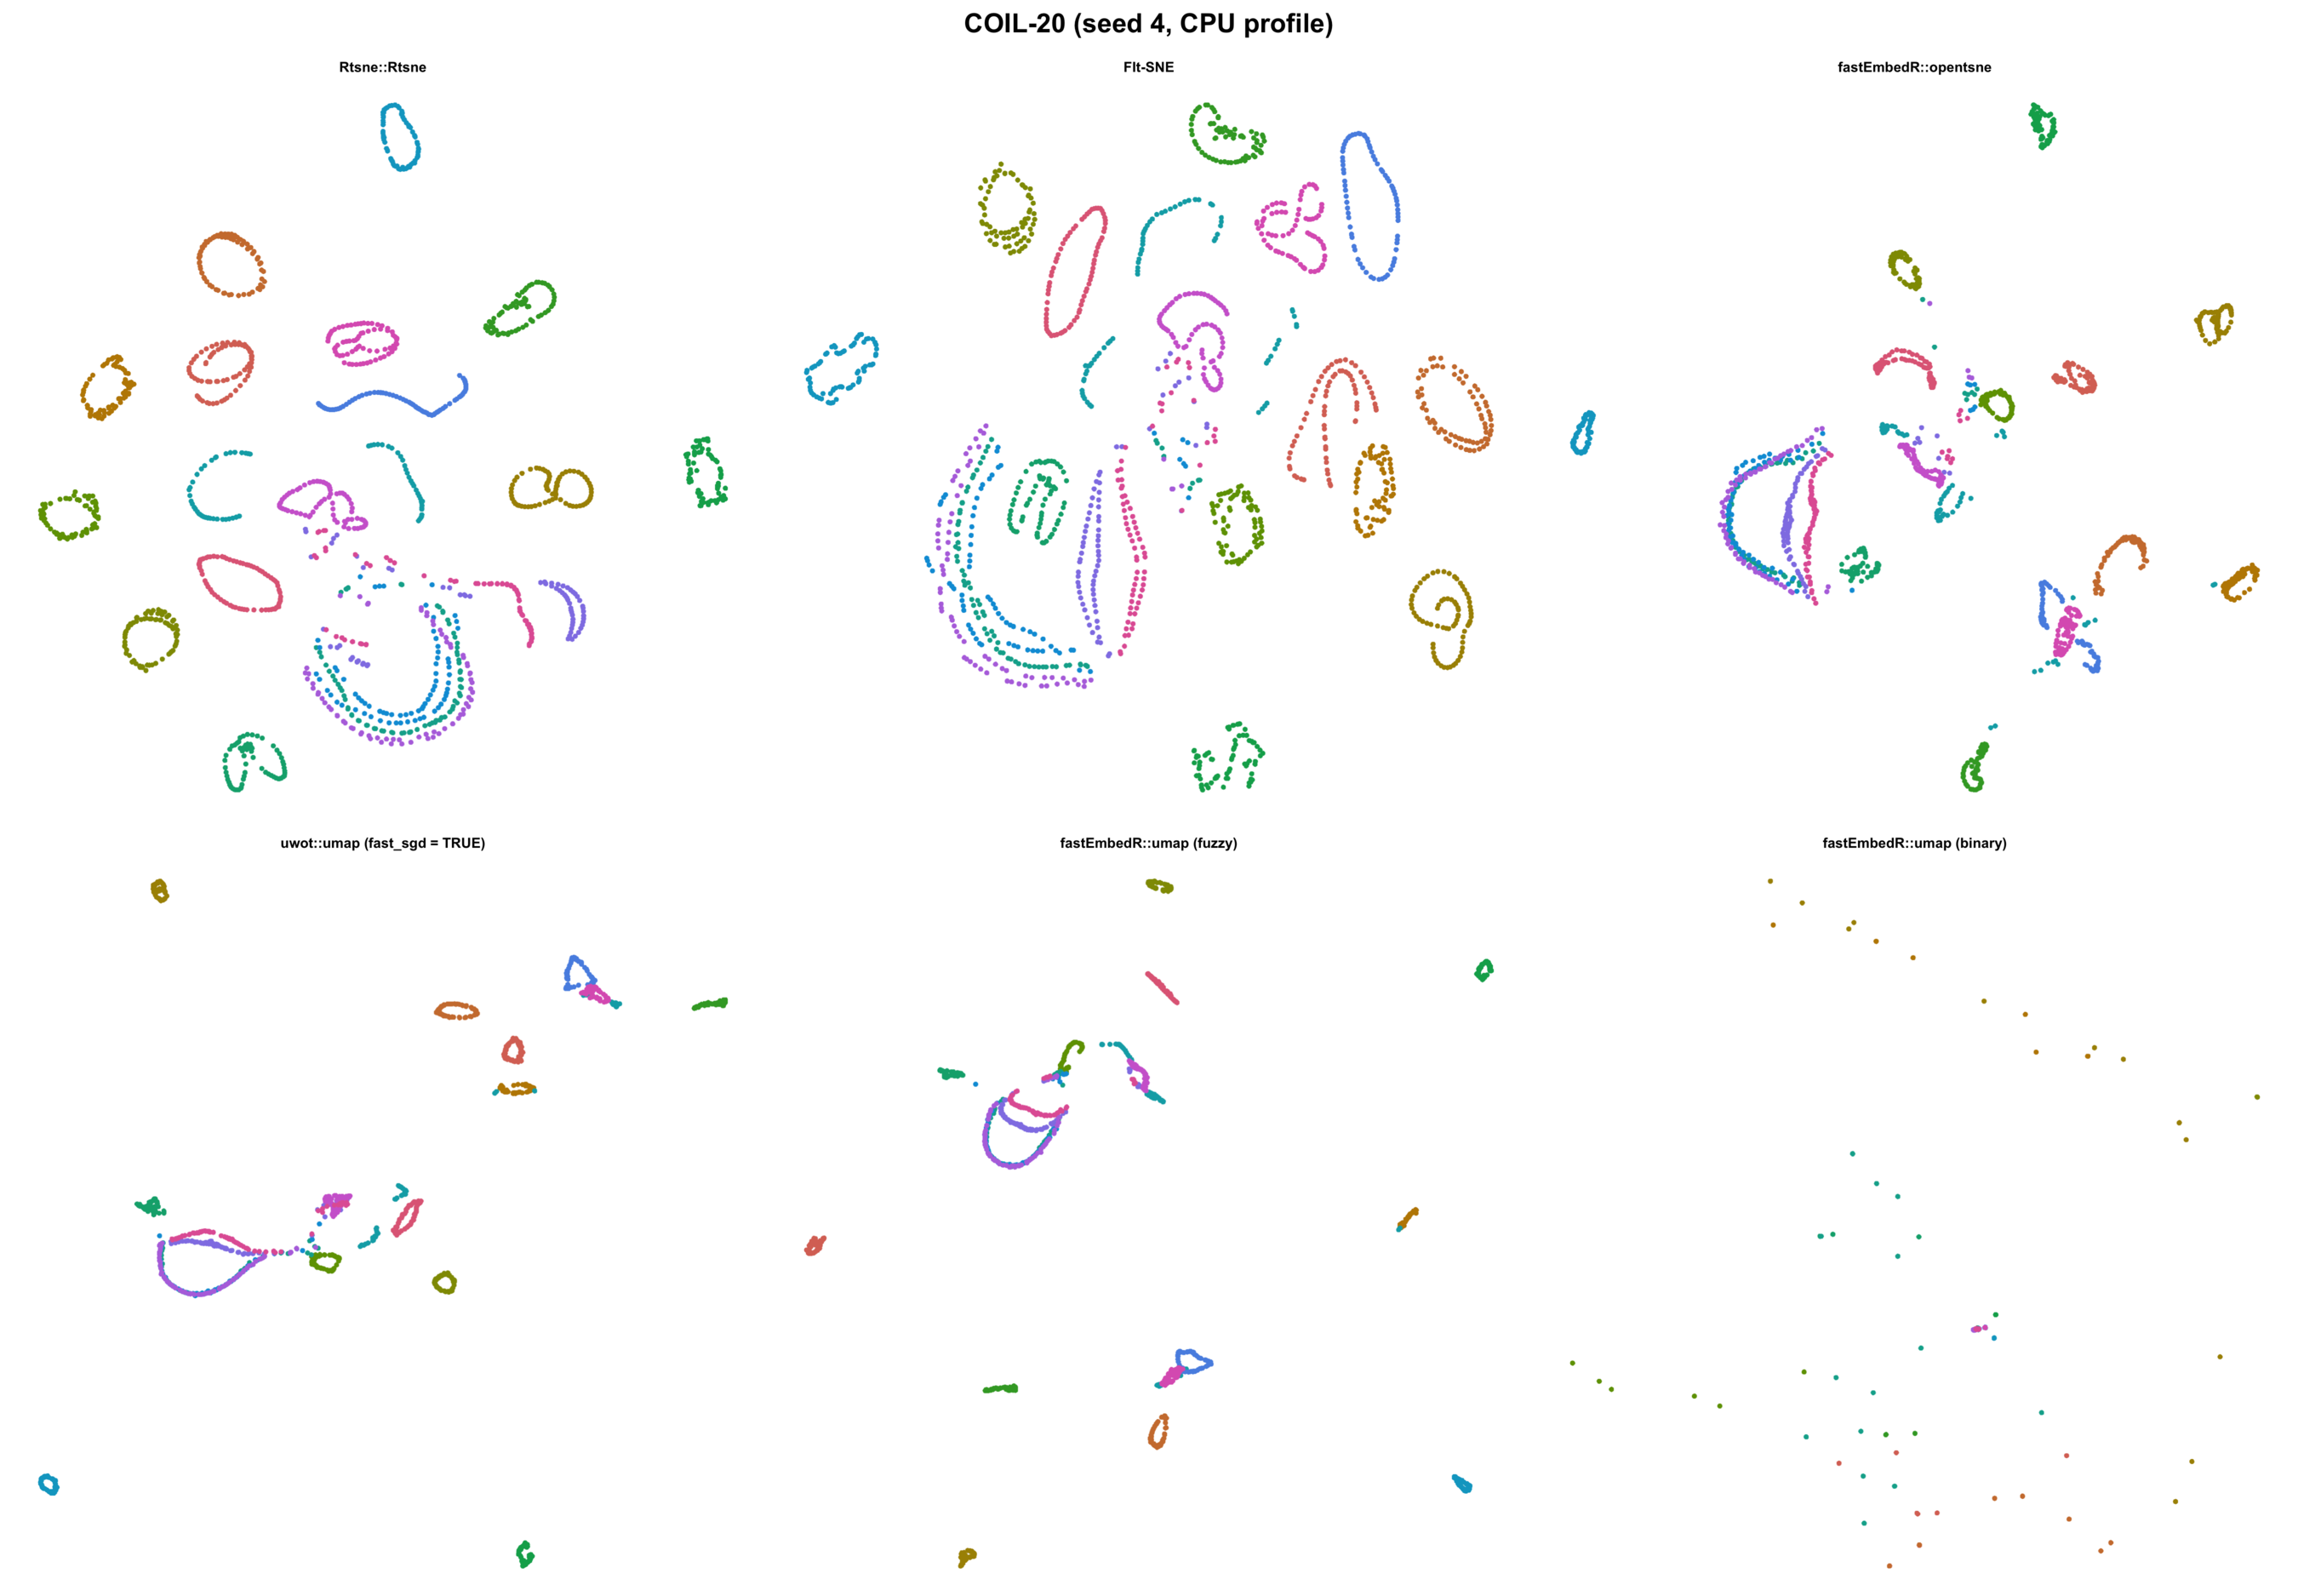
\includegraphics[width=\textwidth]{figures/embedding_comparisons/COIL20_six_methods.png}
\caption{COIL-20 embeddings for the six selected methods (seed 4; CPU profile unless explicitly marked CUDA). The upper row shows Rtsne, FIt-SNE, and \pkg{} openTSNE; the lower row shows uwot UMAP, \pkg{} fuzzy UMAP, and \pkg{} binary UMAP.}
\label{fig:embeddingcoil20}
\end{figure}
\clearpage

\begin{figure}[p]
\centering
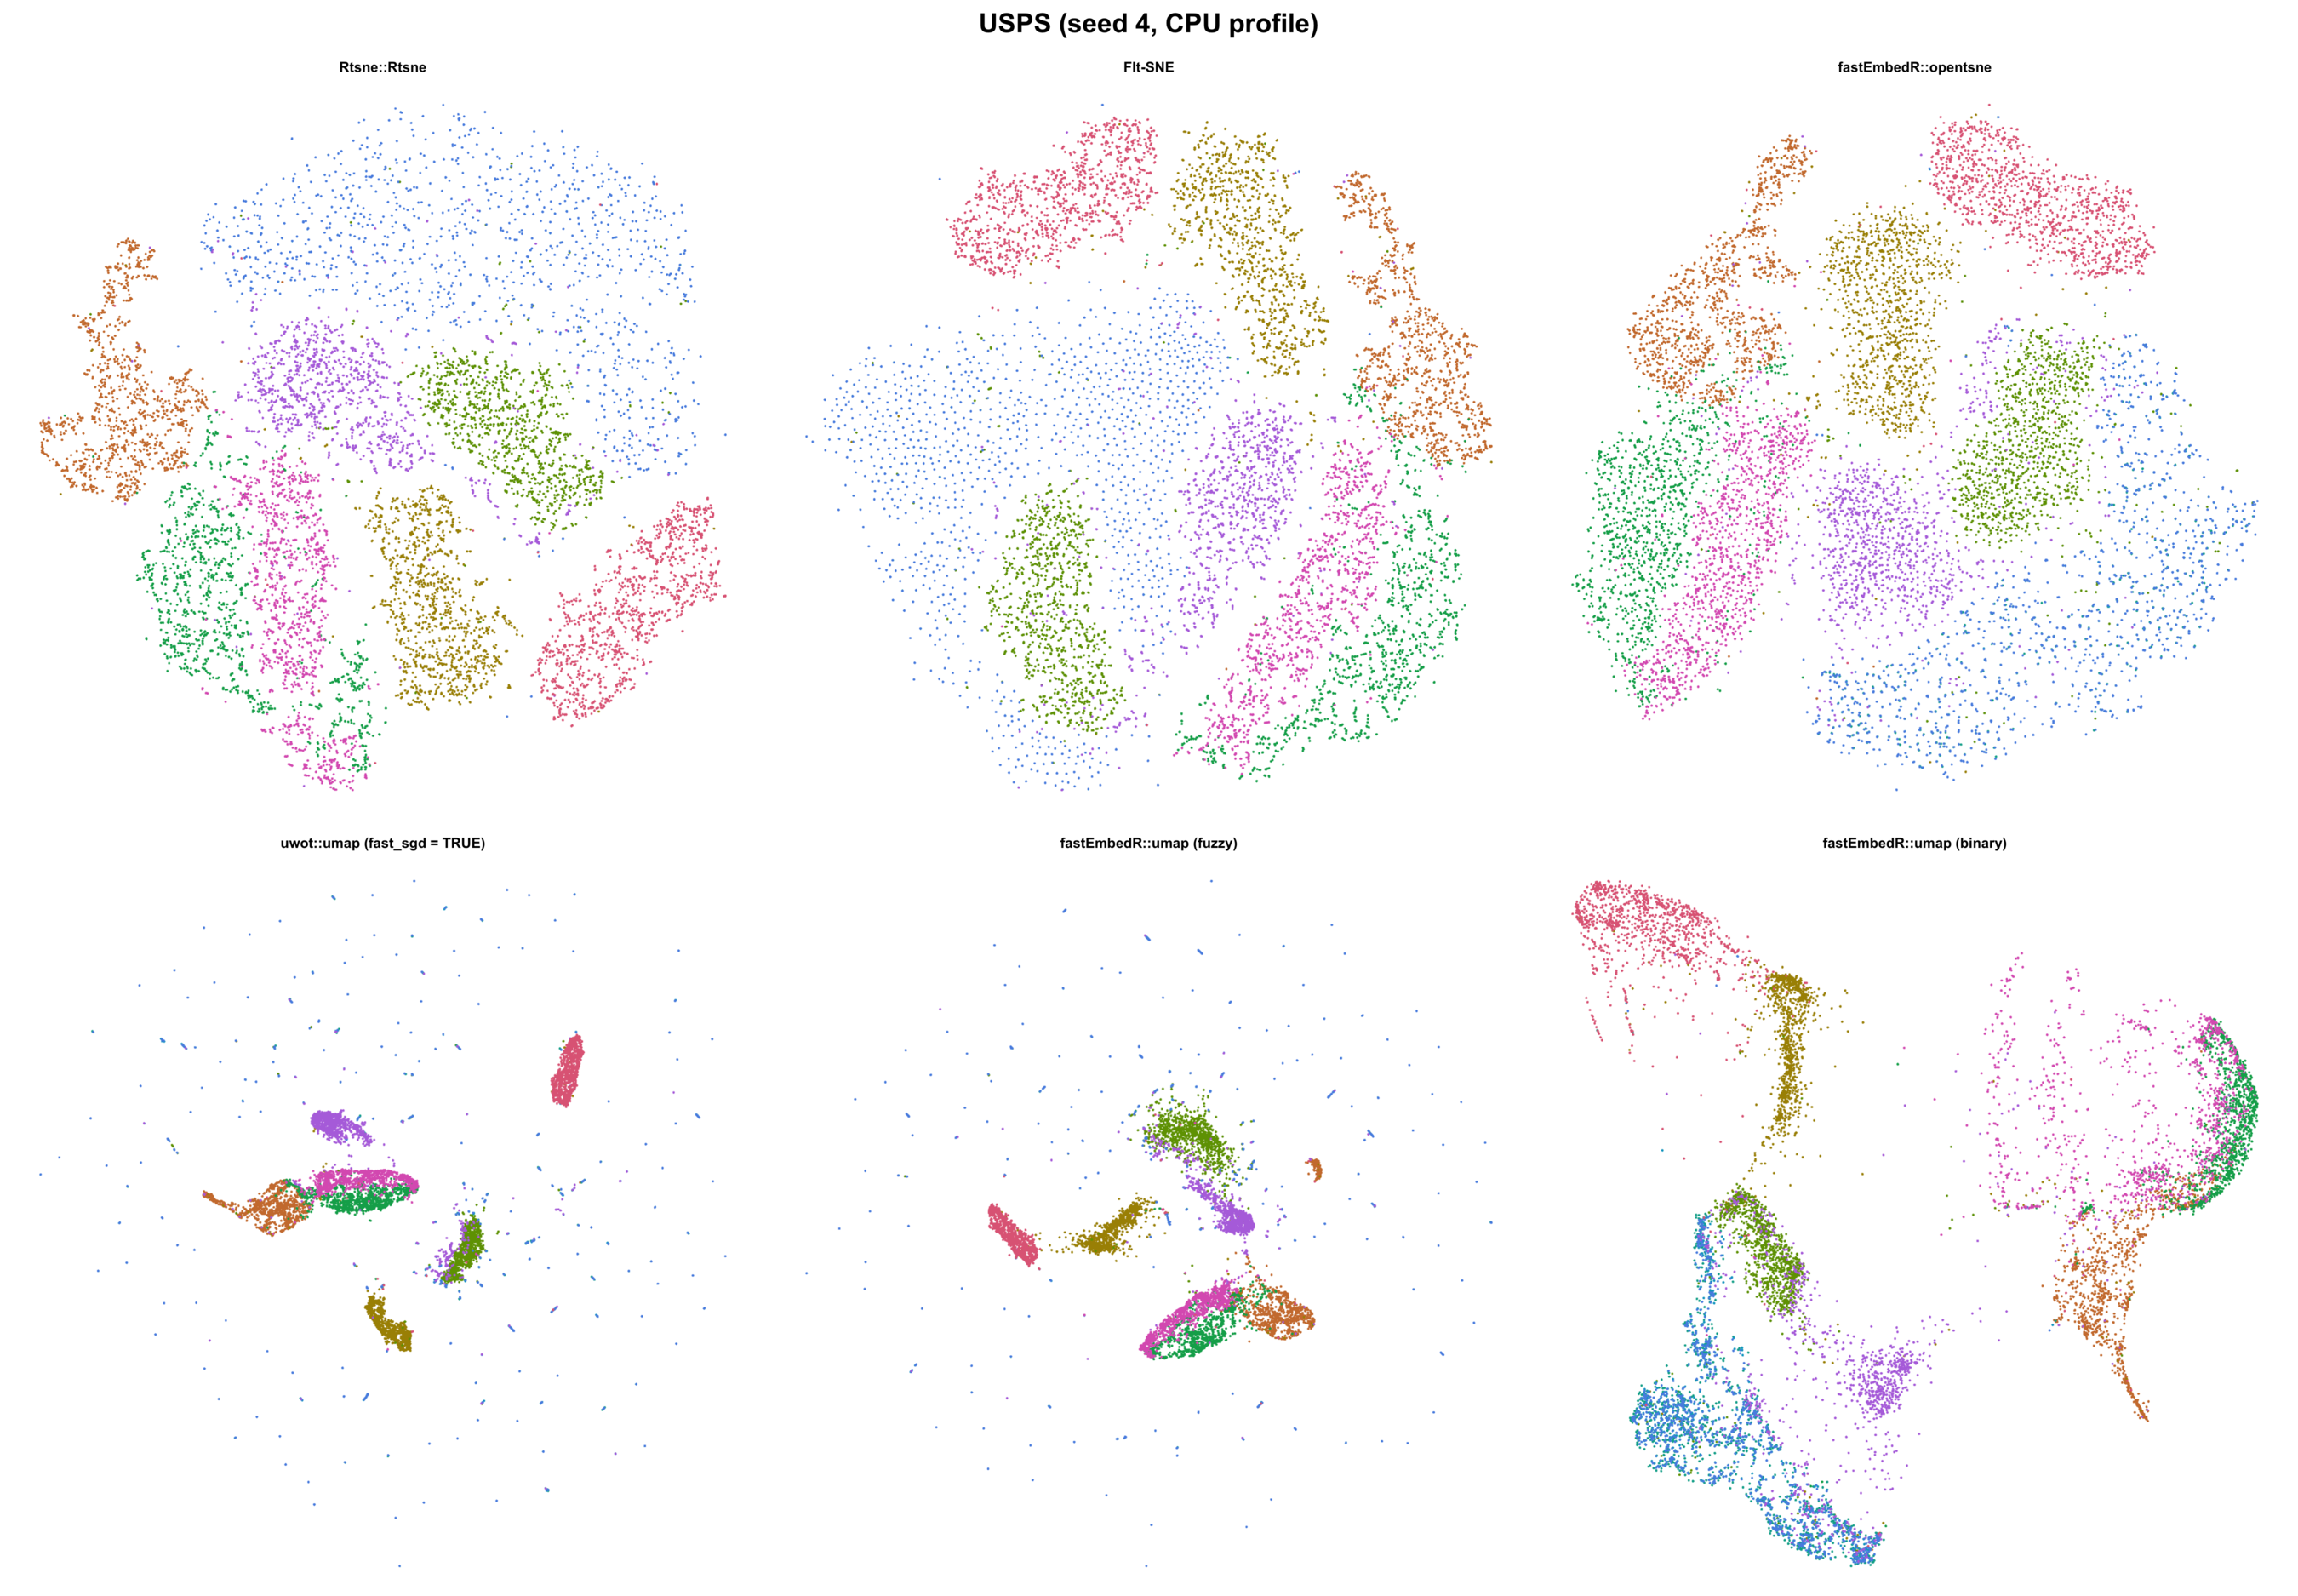
\includegraphics[width=\textwidth]{figures/embedding_comparisons/USPS_six_methods.png}
\caption{USPS embeddings for the six selected methods (seed 4; CPU profile unless explicitly marked CUDA). The upper row shows Rtsne, FIt-SNE, and \pkg{} openTSNE; the lower row shows uwot UMAP, \pkg{} fuzzy UMAP, and \pkg{} binary UMAP.}
\label{fig:embeddingusps}
\end{figure}
\clearpage

\begin{figure}[p]
\centering
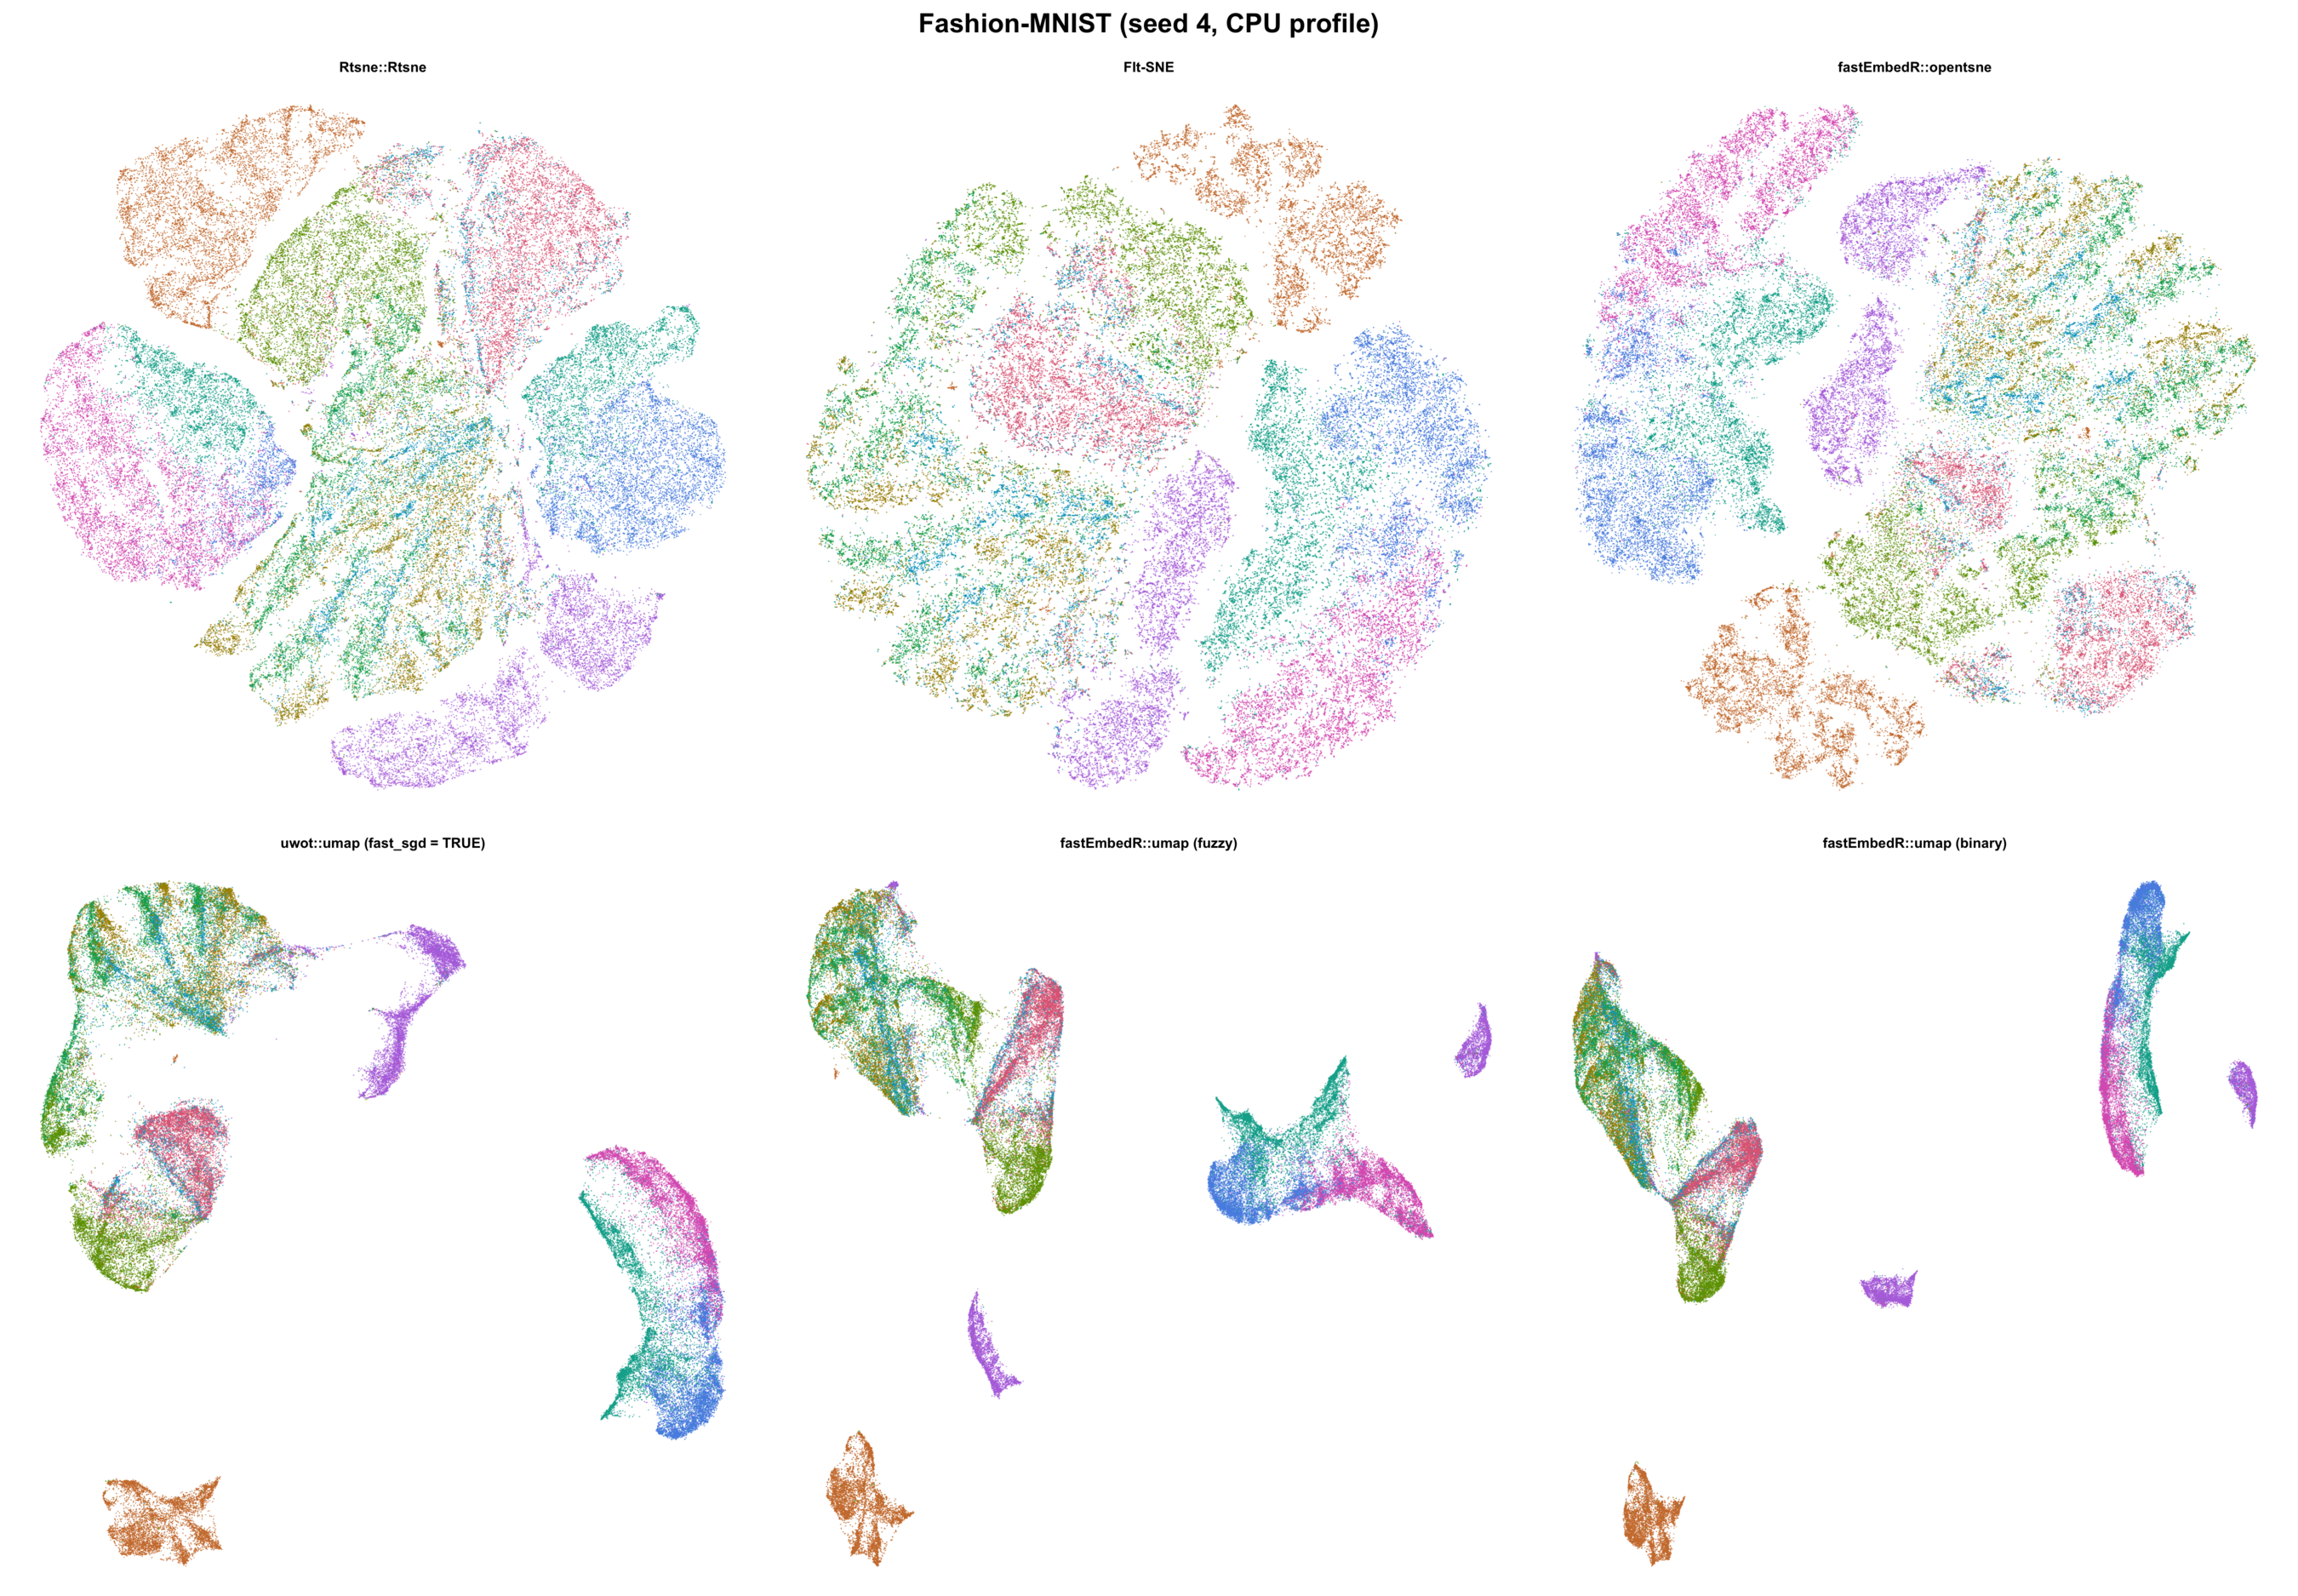
\includegraphics[width=\textwidth]{figures/embedding_comparisons/FashionMNIST_six_methods.png}
\caption{Fashion-MNIST embeddings for the six selected methods (seed 4; CPU profile unless explicitly marked CUDA). The upper row shows Rtsne, FIt-SNE, and \pkg{} openTSNE; the lower row shows uwot UMAP, \pkg{} fuzzy UMAP, and \pkg{} binary UMAP.}
\label{fig:embeddingfashionmnist}
\end{figure}
\clearpage

\begin{figure}[p]
\centering
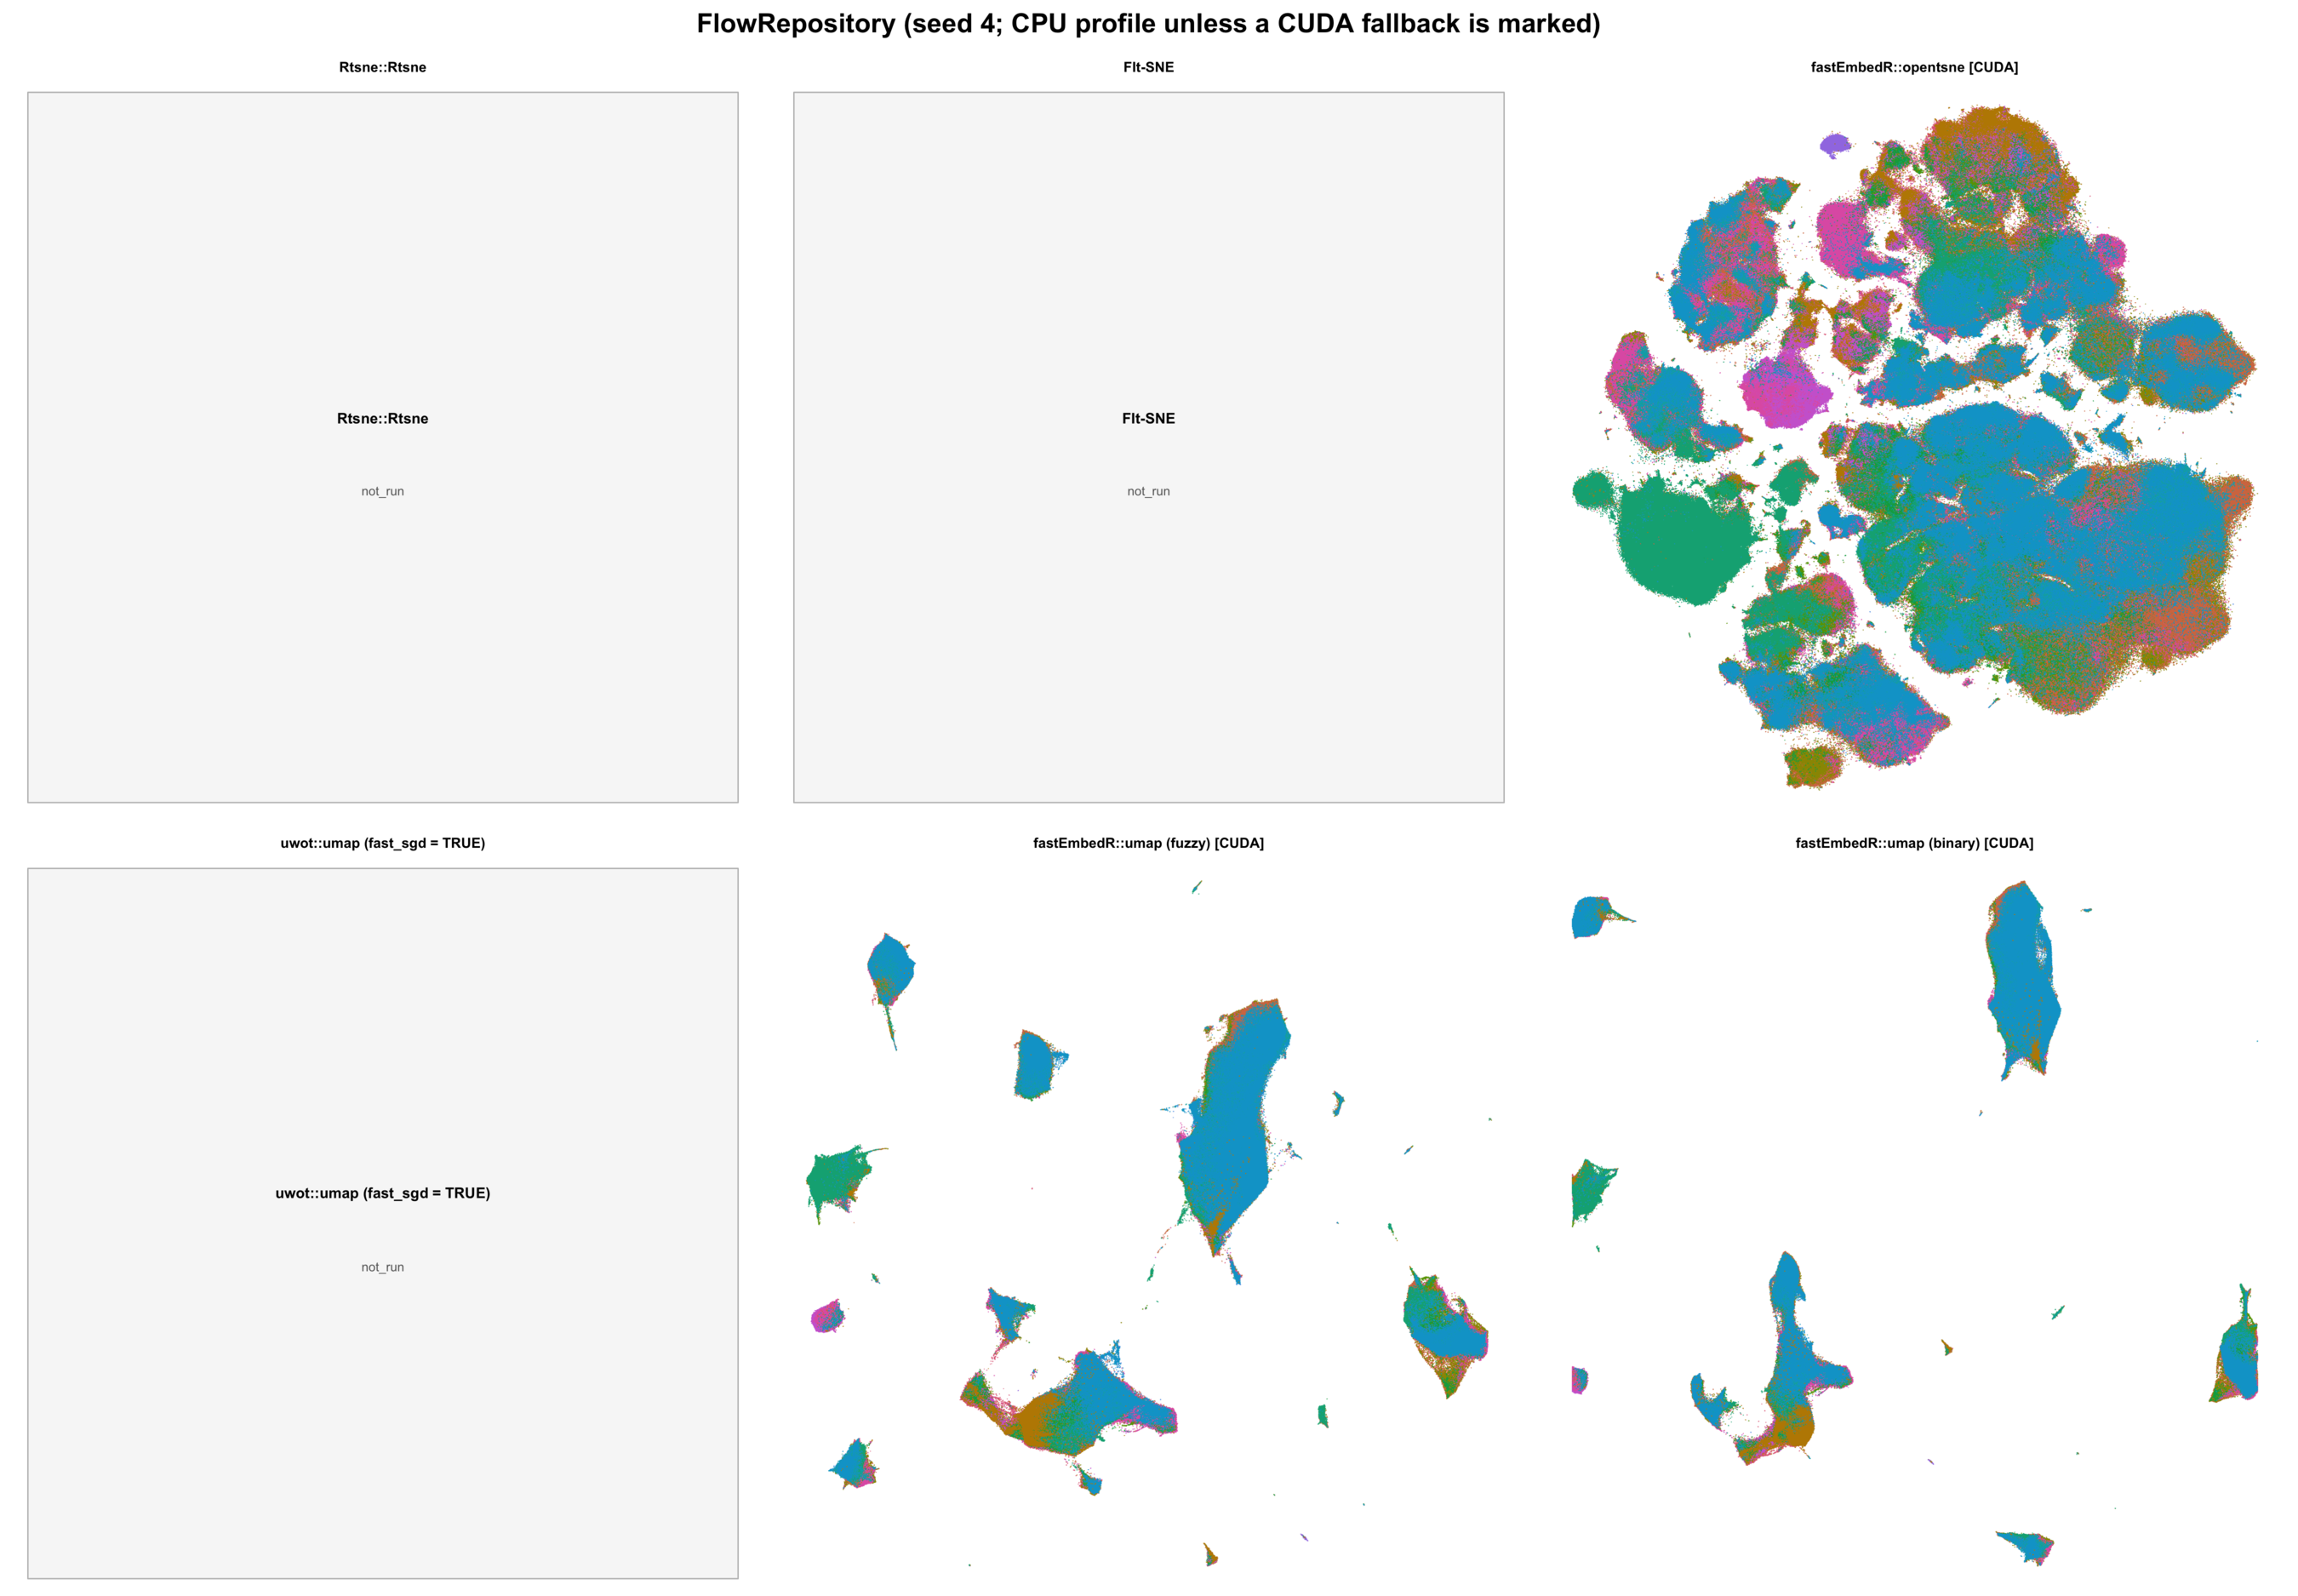
\includegraphics[width=\textwidth]{figures/embedding_comparisons/FlowRepository_FR_FCM_ZYRM_files_six_methods.png}
\caption{FlowRepository embeddings for the six selected methods (seed 4; CPU profile unless explicitly marked CUDA). The upper row shows Rtsne, FIt-SNE, and \pkg{} openTSNE; the lower row shows uwot UMAP, \pkg{} fuzzy UMAP, and \pkg{} binary UMAP. This dataset has no successful matched reference row; displayed fastEmbedR results are descriptive only.}
\label{fig:embeddingflowrepositoryfrfcmzyrmfiles}
\end{figure}
\clearpage

\begin{figure}[p]
\centering
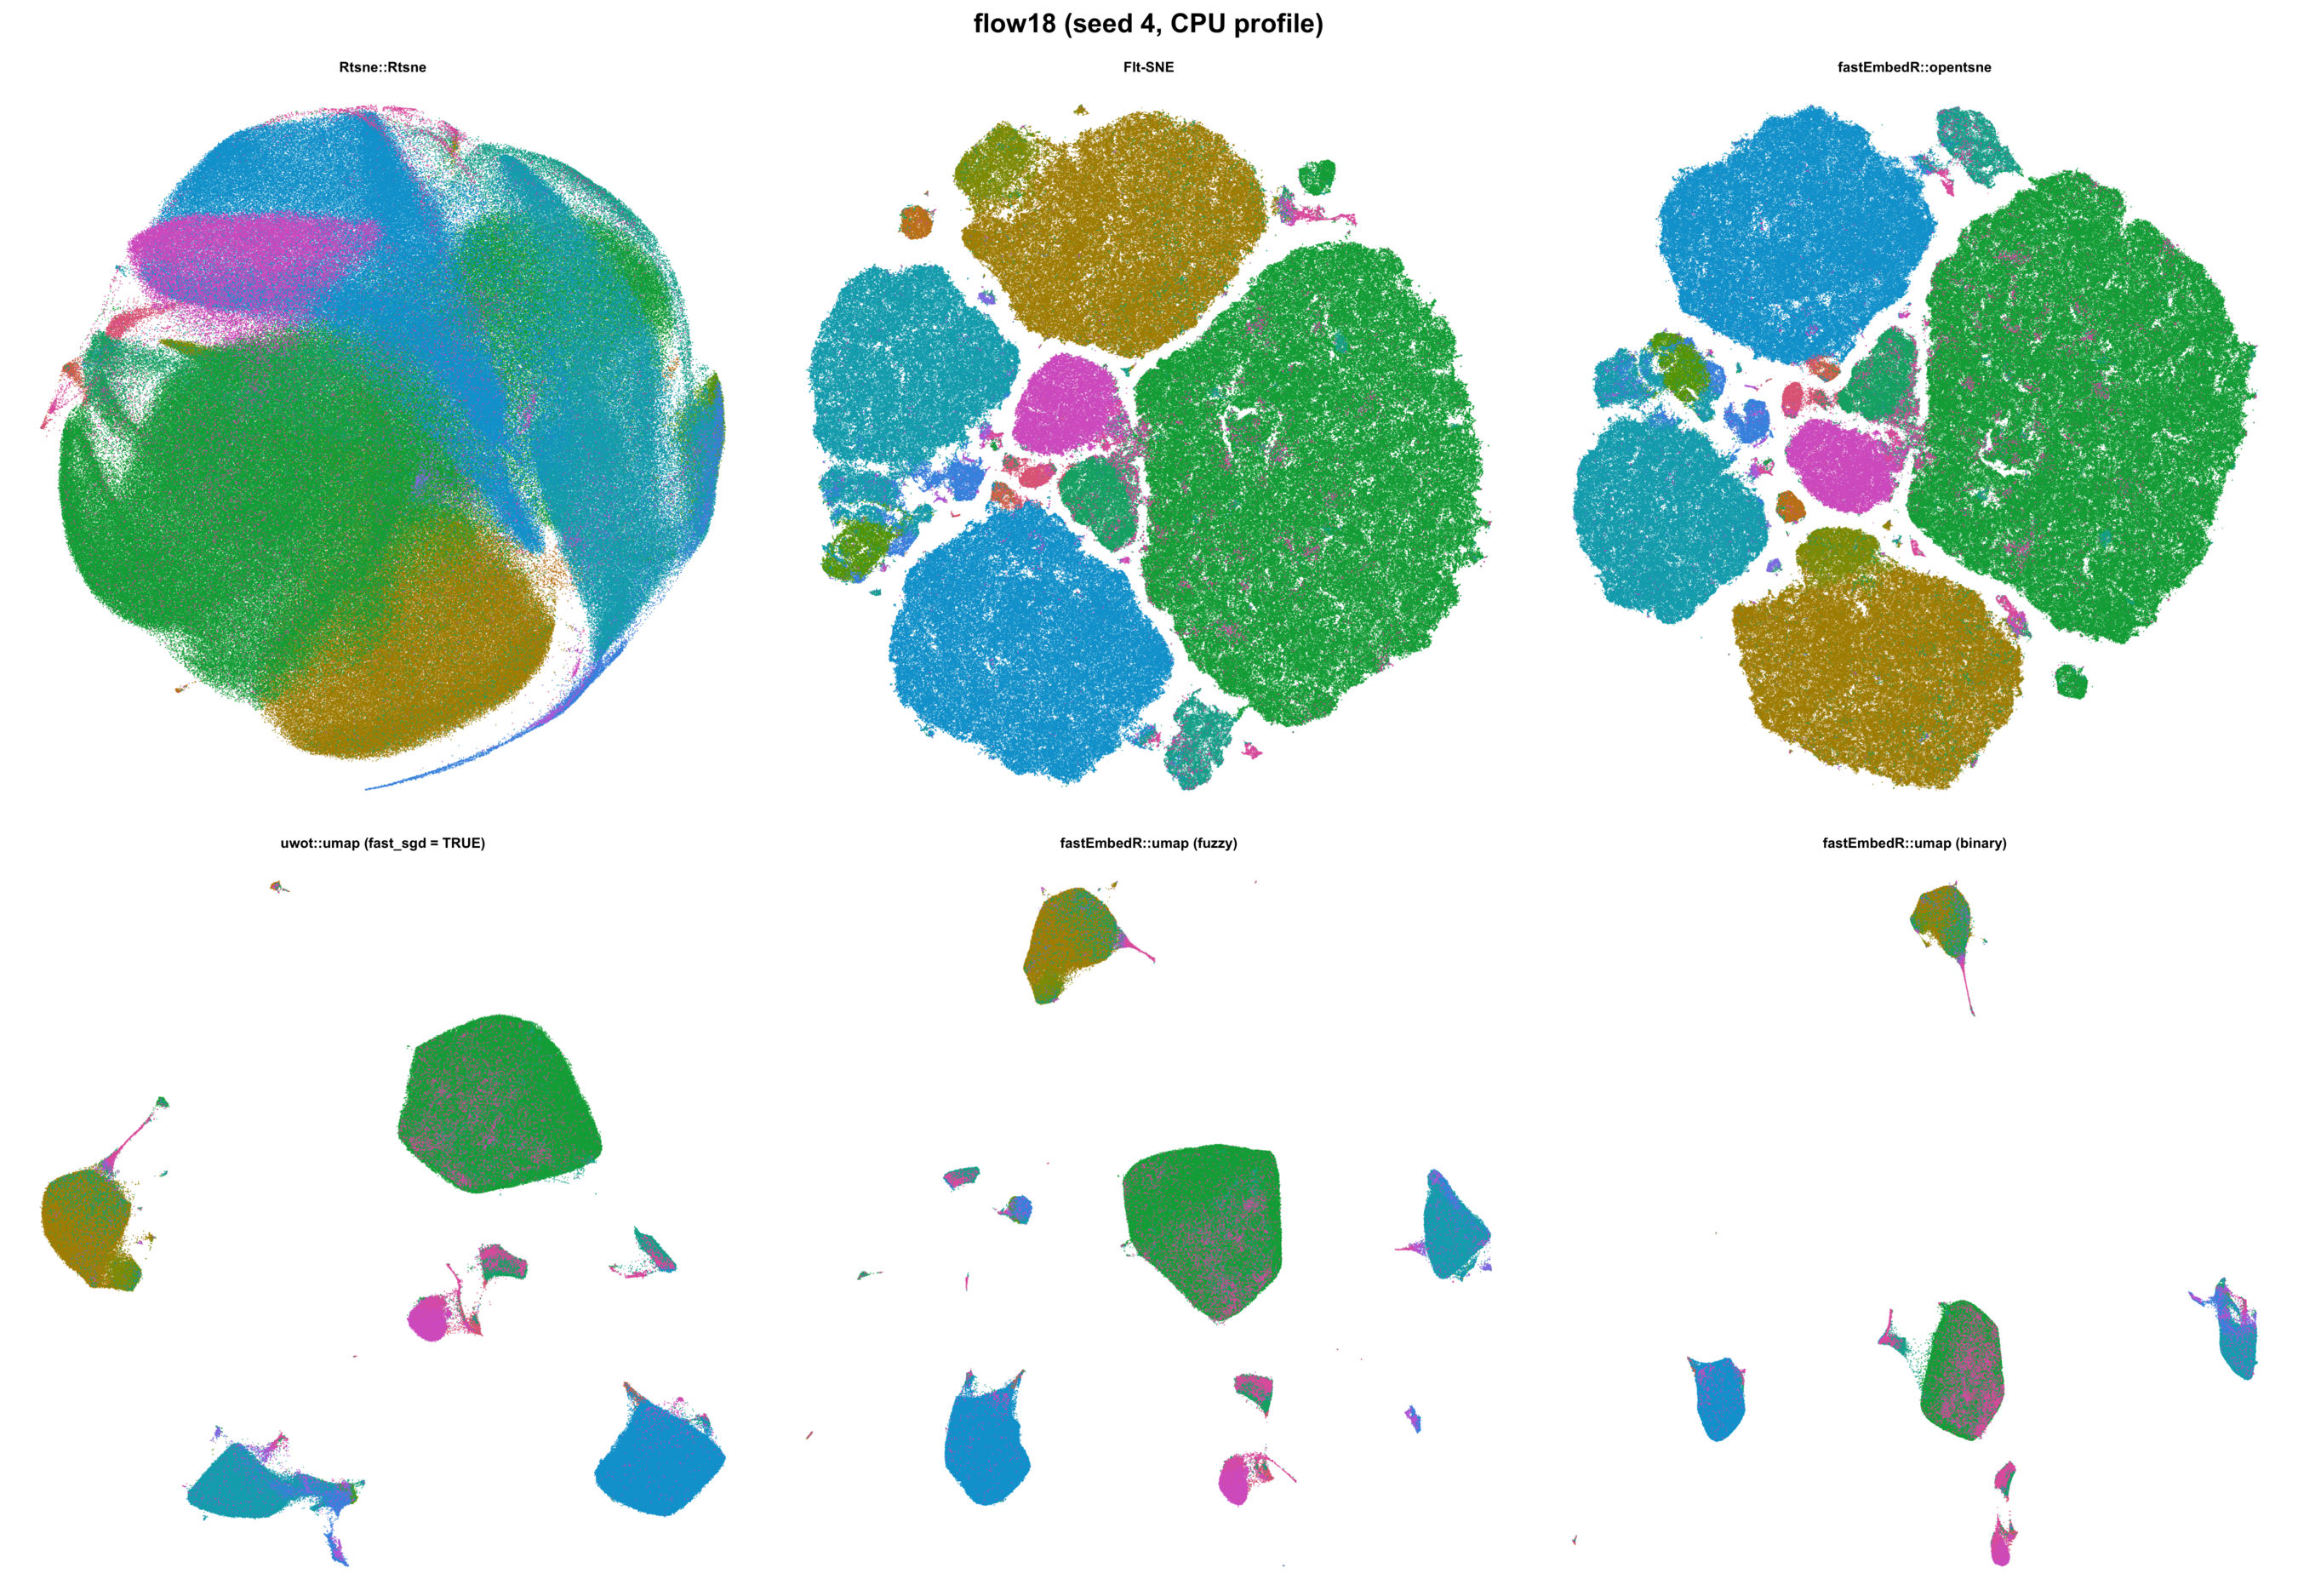
\includegraphics[width=\textwidth]{figures/embedding_comparisons/flow18_six_methods.png}
\caption{flow18 embeddings for the six selected methods (seed 4; CPU profile unless explicitly marked CUDA). The upper row shows Rtsne, FIt-SNE, and \pkg{} openTSNE; the lower row shows uwot UMAP, \pkg{} fuzzy UMAP, and \pkg{} binary UMAP.}
\label{fig:embeddingflow18}
\end{figure}
\clearpage

\begin{figure}[p]
\centering
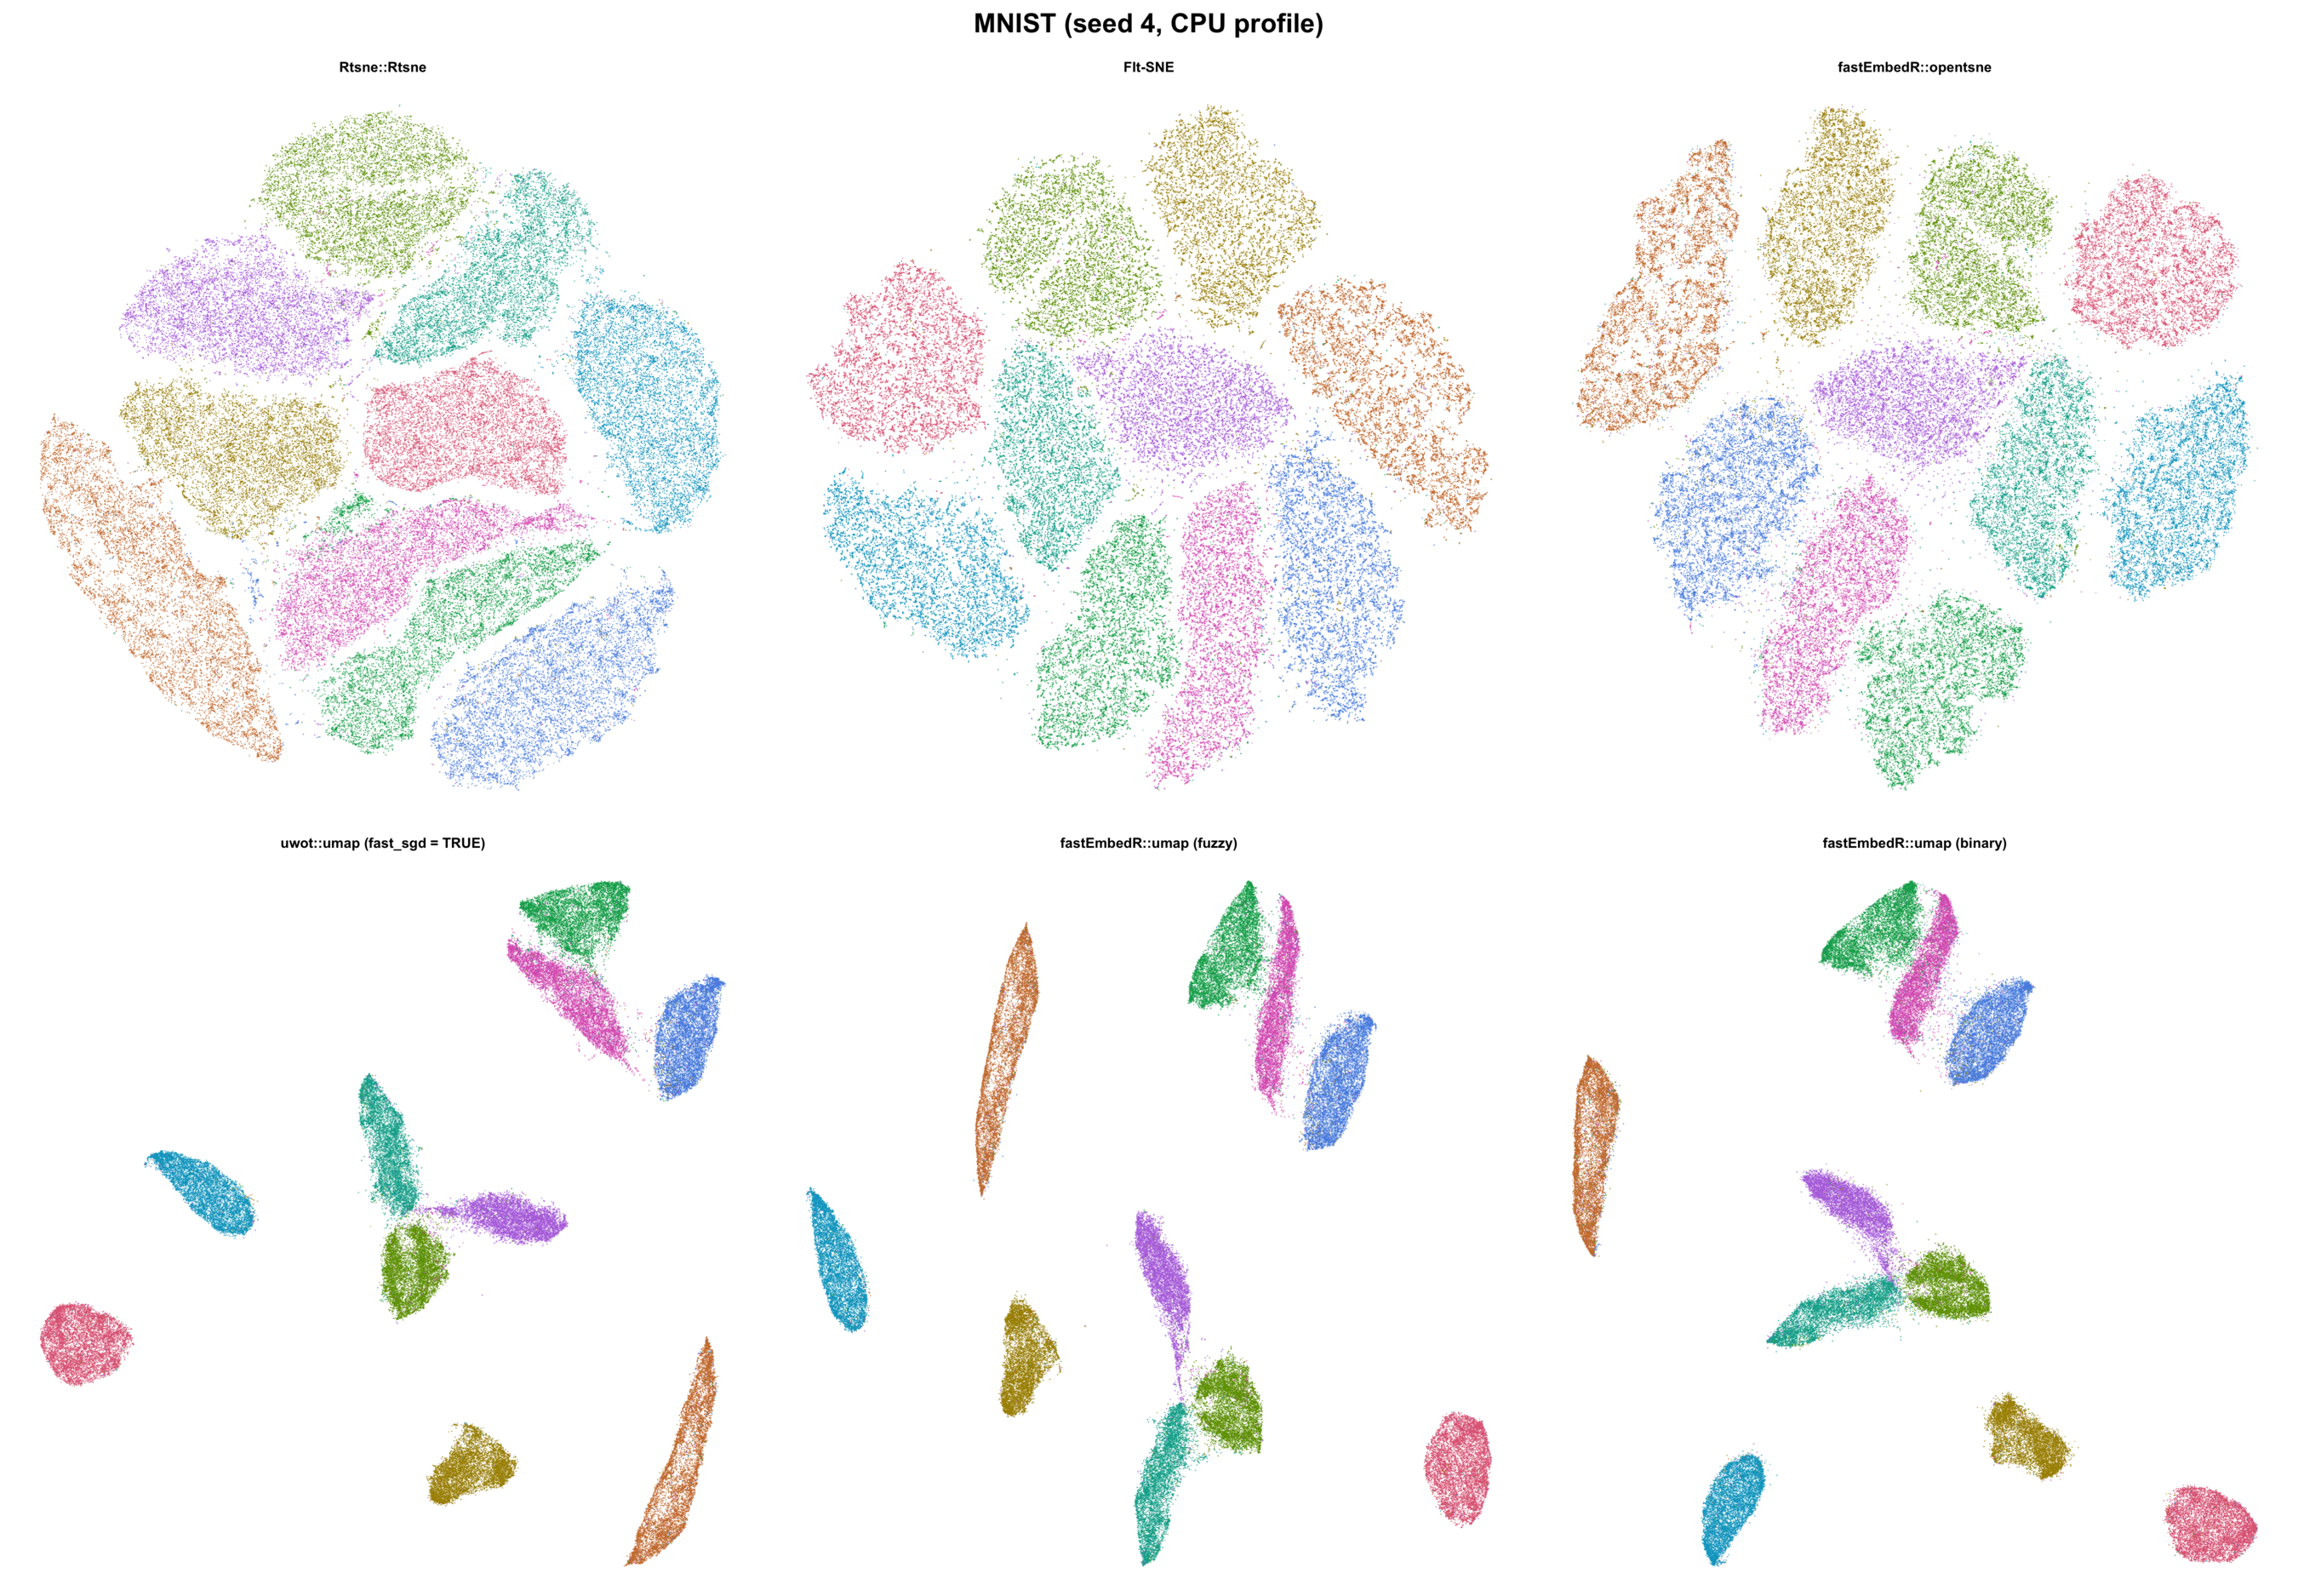
\includegraphics[width=\textwidth]{figures/embedding_comparisons/MNIST_six_methods.png}
\caption{MNIST embeddings for the six selected methods (seed 4; CPU profile unless explicitly marked CUDA). The upper row shows Rtsne, FIt-SNE, and \pkg{} openTSNE; the lower row shows uwot UMAP, \pkg{} fuzzy UMAP, and \pkg{} binary UMAP.}
\label{fig:embeddingmnist}
\end{figure}
\clearpage

\begin{figure}[p]
\centering
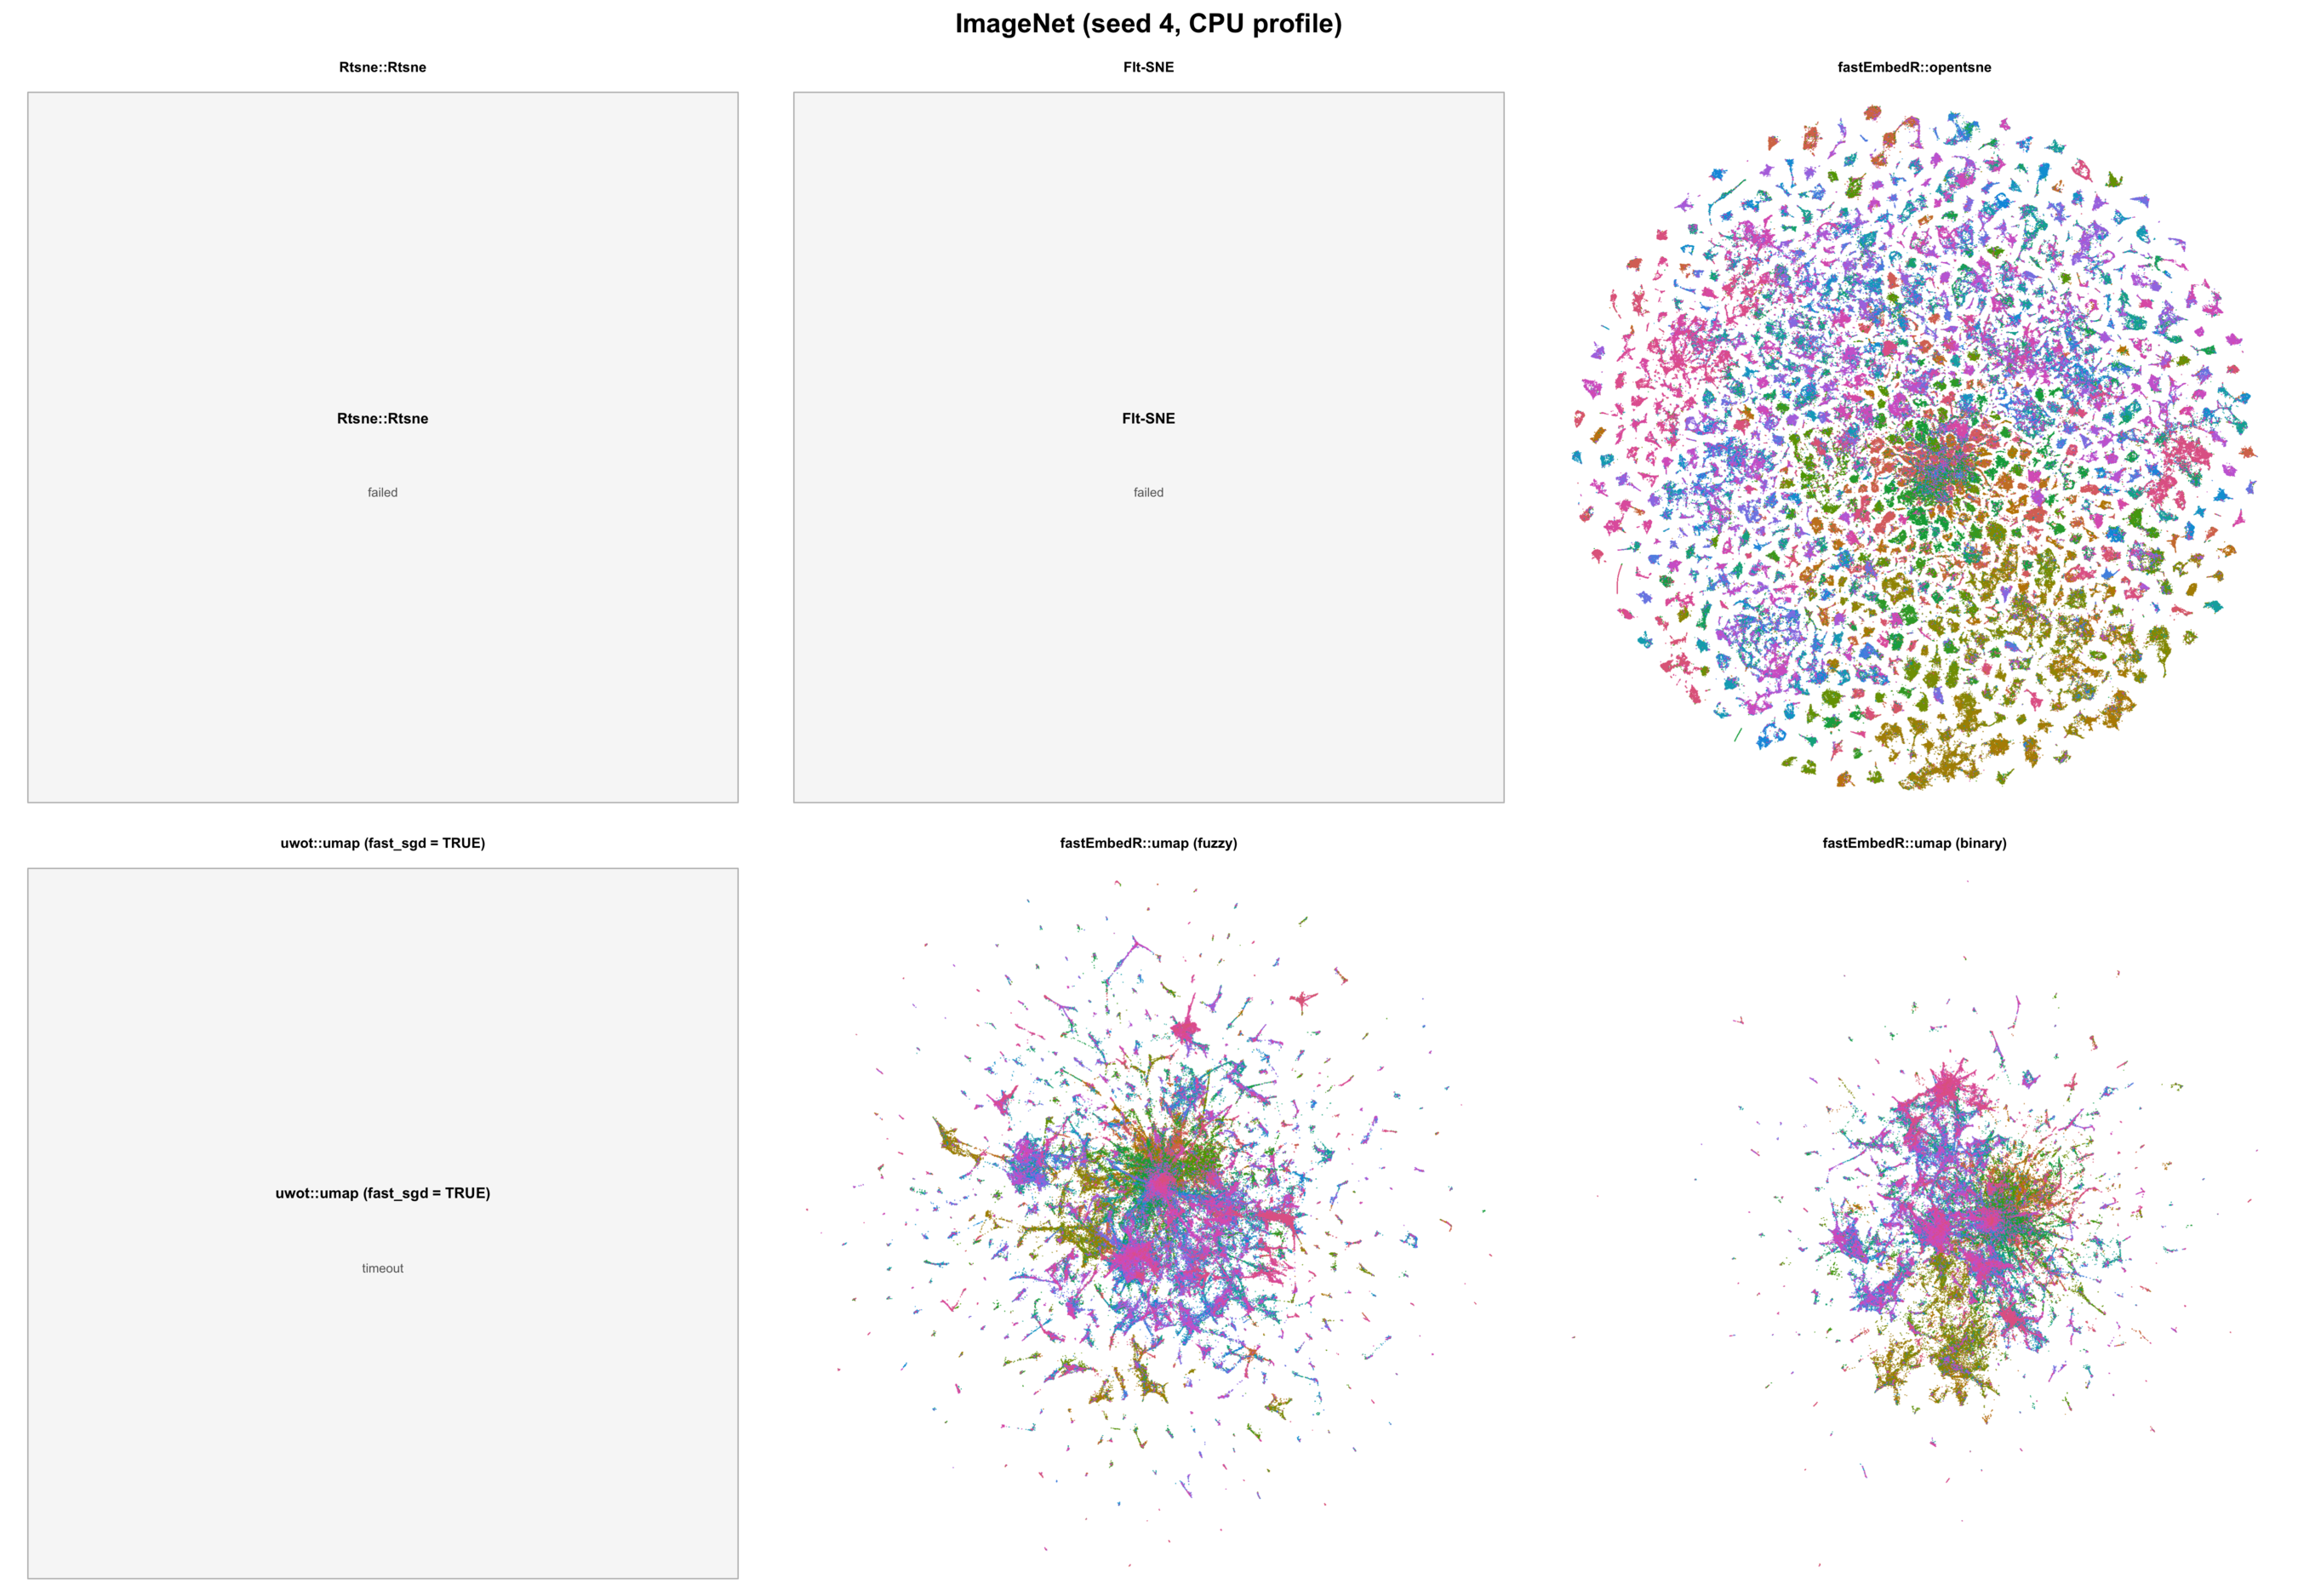
\includegraphics[width=\textwidth]{figures/embedding_comparisons/imagenet_six_methods.png}
\caption{ImageNet embeddings for the six selected methods (seed 4; CPU profile unless explicitly marked CUDA). The upper row shows Rtsne, FIt-SNE, and \pkg{} openTSNE; the lower row shows uwot UMAP, \pkg{} fuzzy UMAP, and \pkg{} binary UMAP. This dataset has no successful matched reference row; displayed fastEmbedR results are descriptive only.}
\label{fig:embeddingimagenet}
\end{figure}
\clearpage

\begin{figure}[p]
\centering
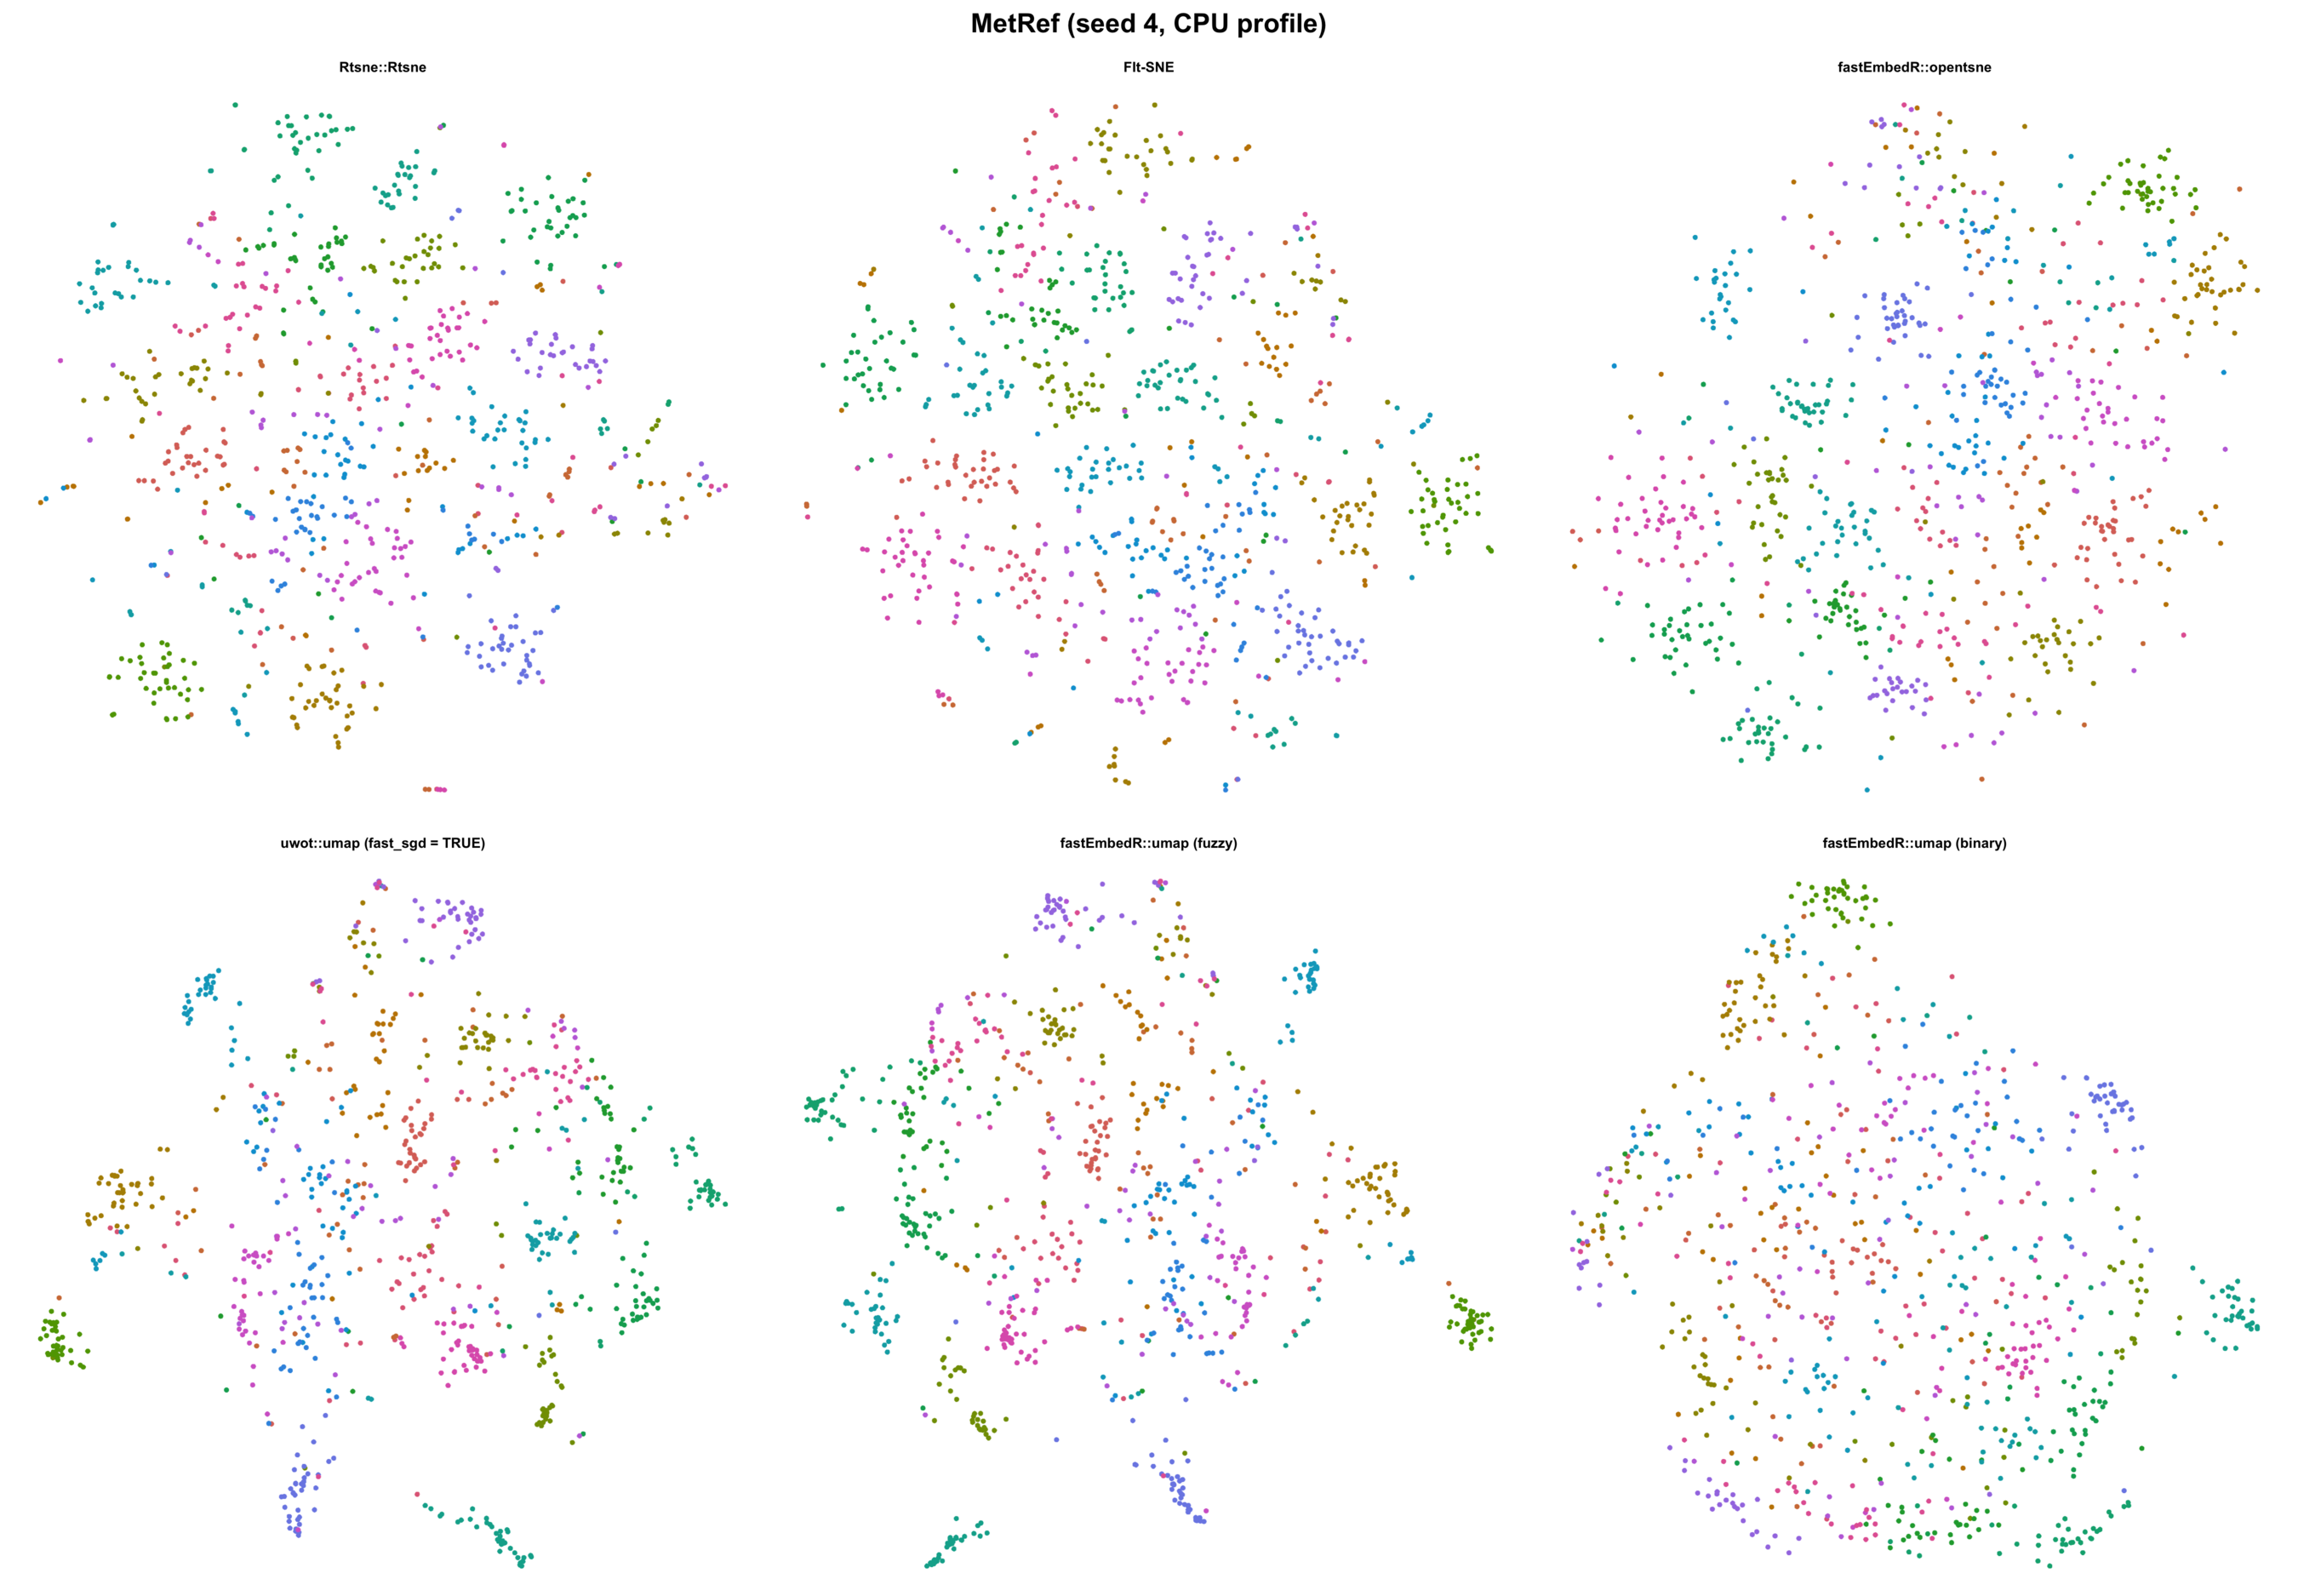
\includegraphics[width=\textwidth]{figures/embedding_comparisons/MetRef_six_methods.png}
\caption{MetRef embeddings for the six selected methods (seed 4; CPU profile unless explicitly marked CUDA). The upper row shows Rtsne, FIt-SNE, and \pkg{} openTSNE; the lower row shows uwot UMAP, \pkg{} fuzzy UMAP, and \pkg{} binary UMAP.}
\label{fig:embeddingmetref}
\end{figure}
\clearpage

\begin{figure}[p]
\centering
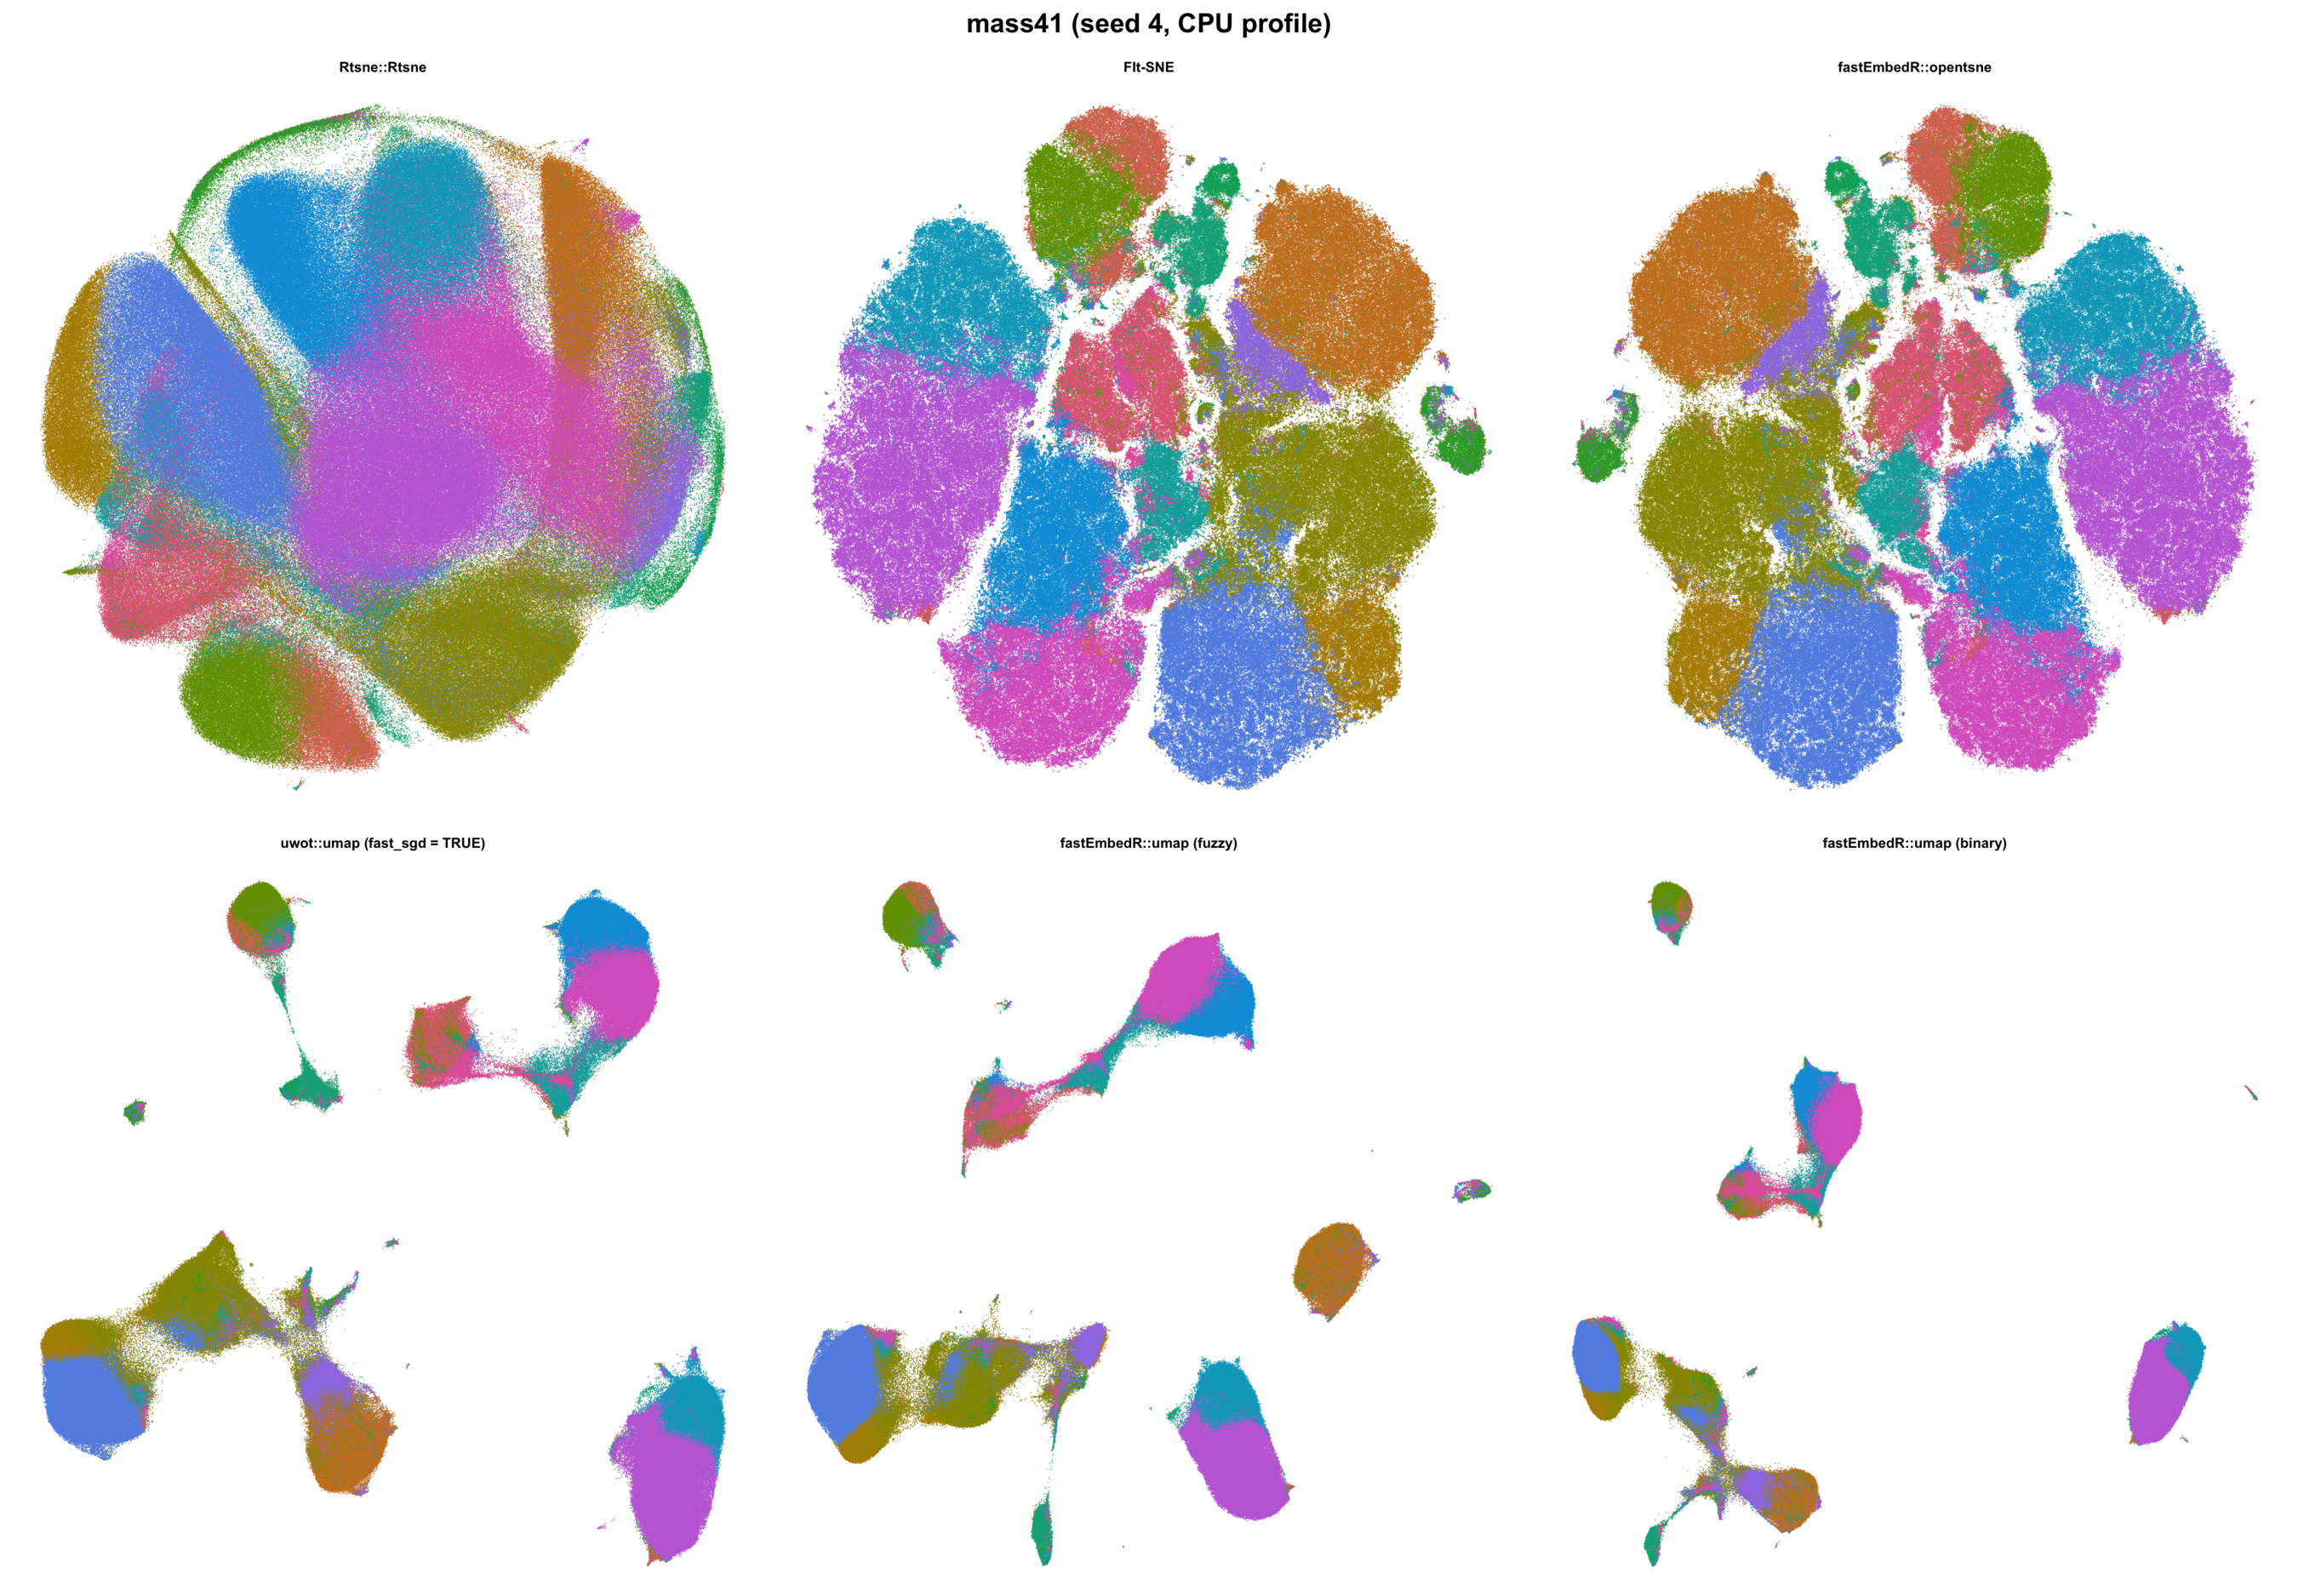
\includegraphics[width=\textwidth]{figures/embedding_comparisons/mass41_six_methods.png}
\caption{mass41 embeddings for the six selected methods (seed 4; CPU profile unless explicitly marked CUDA). The upper row shows Rtsne, FIt-SNE, and \pkg{} openTSNE; the lower row shows uwot UMAP, \pkg{} fuzzy UMAP, and \pkg{} binary UMAP.}
\label{fig:embeddingmass41}
\end{figure}
\clearpage

\begin{figure}[p]
\centering
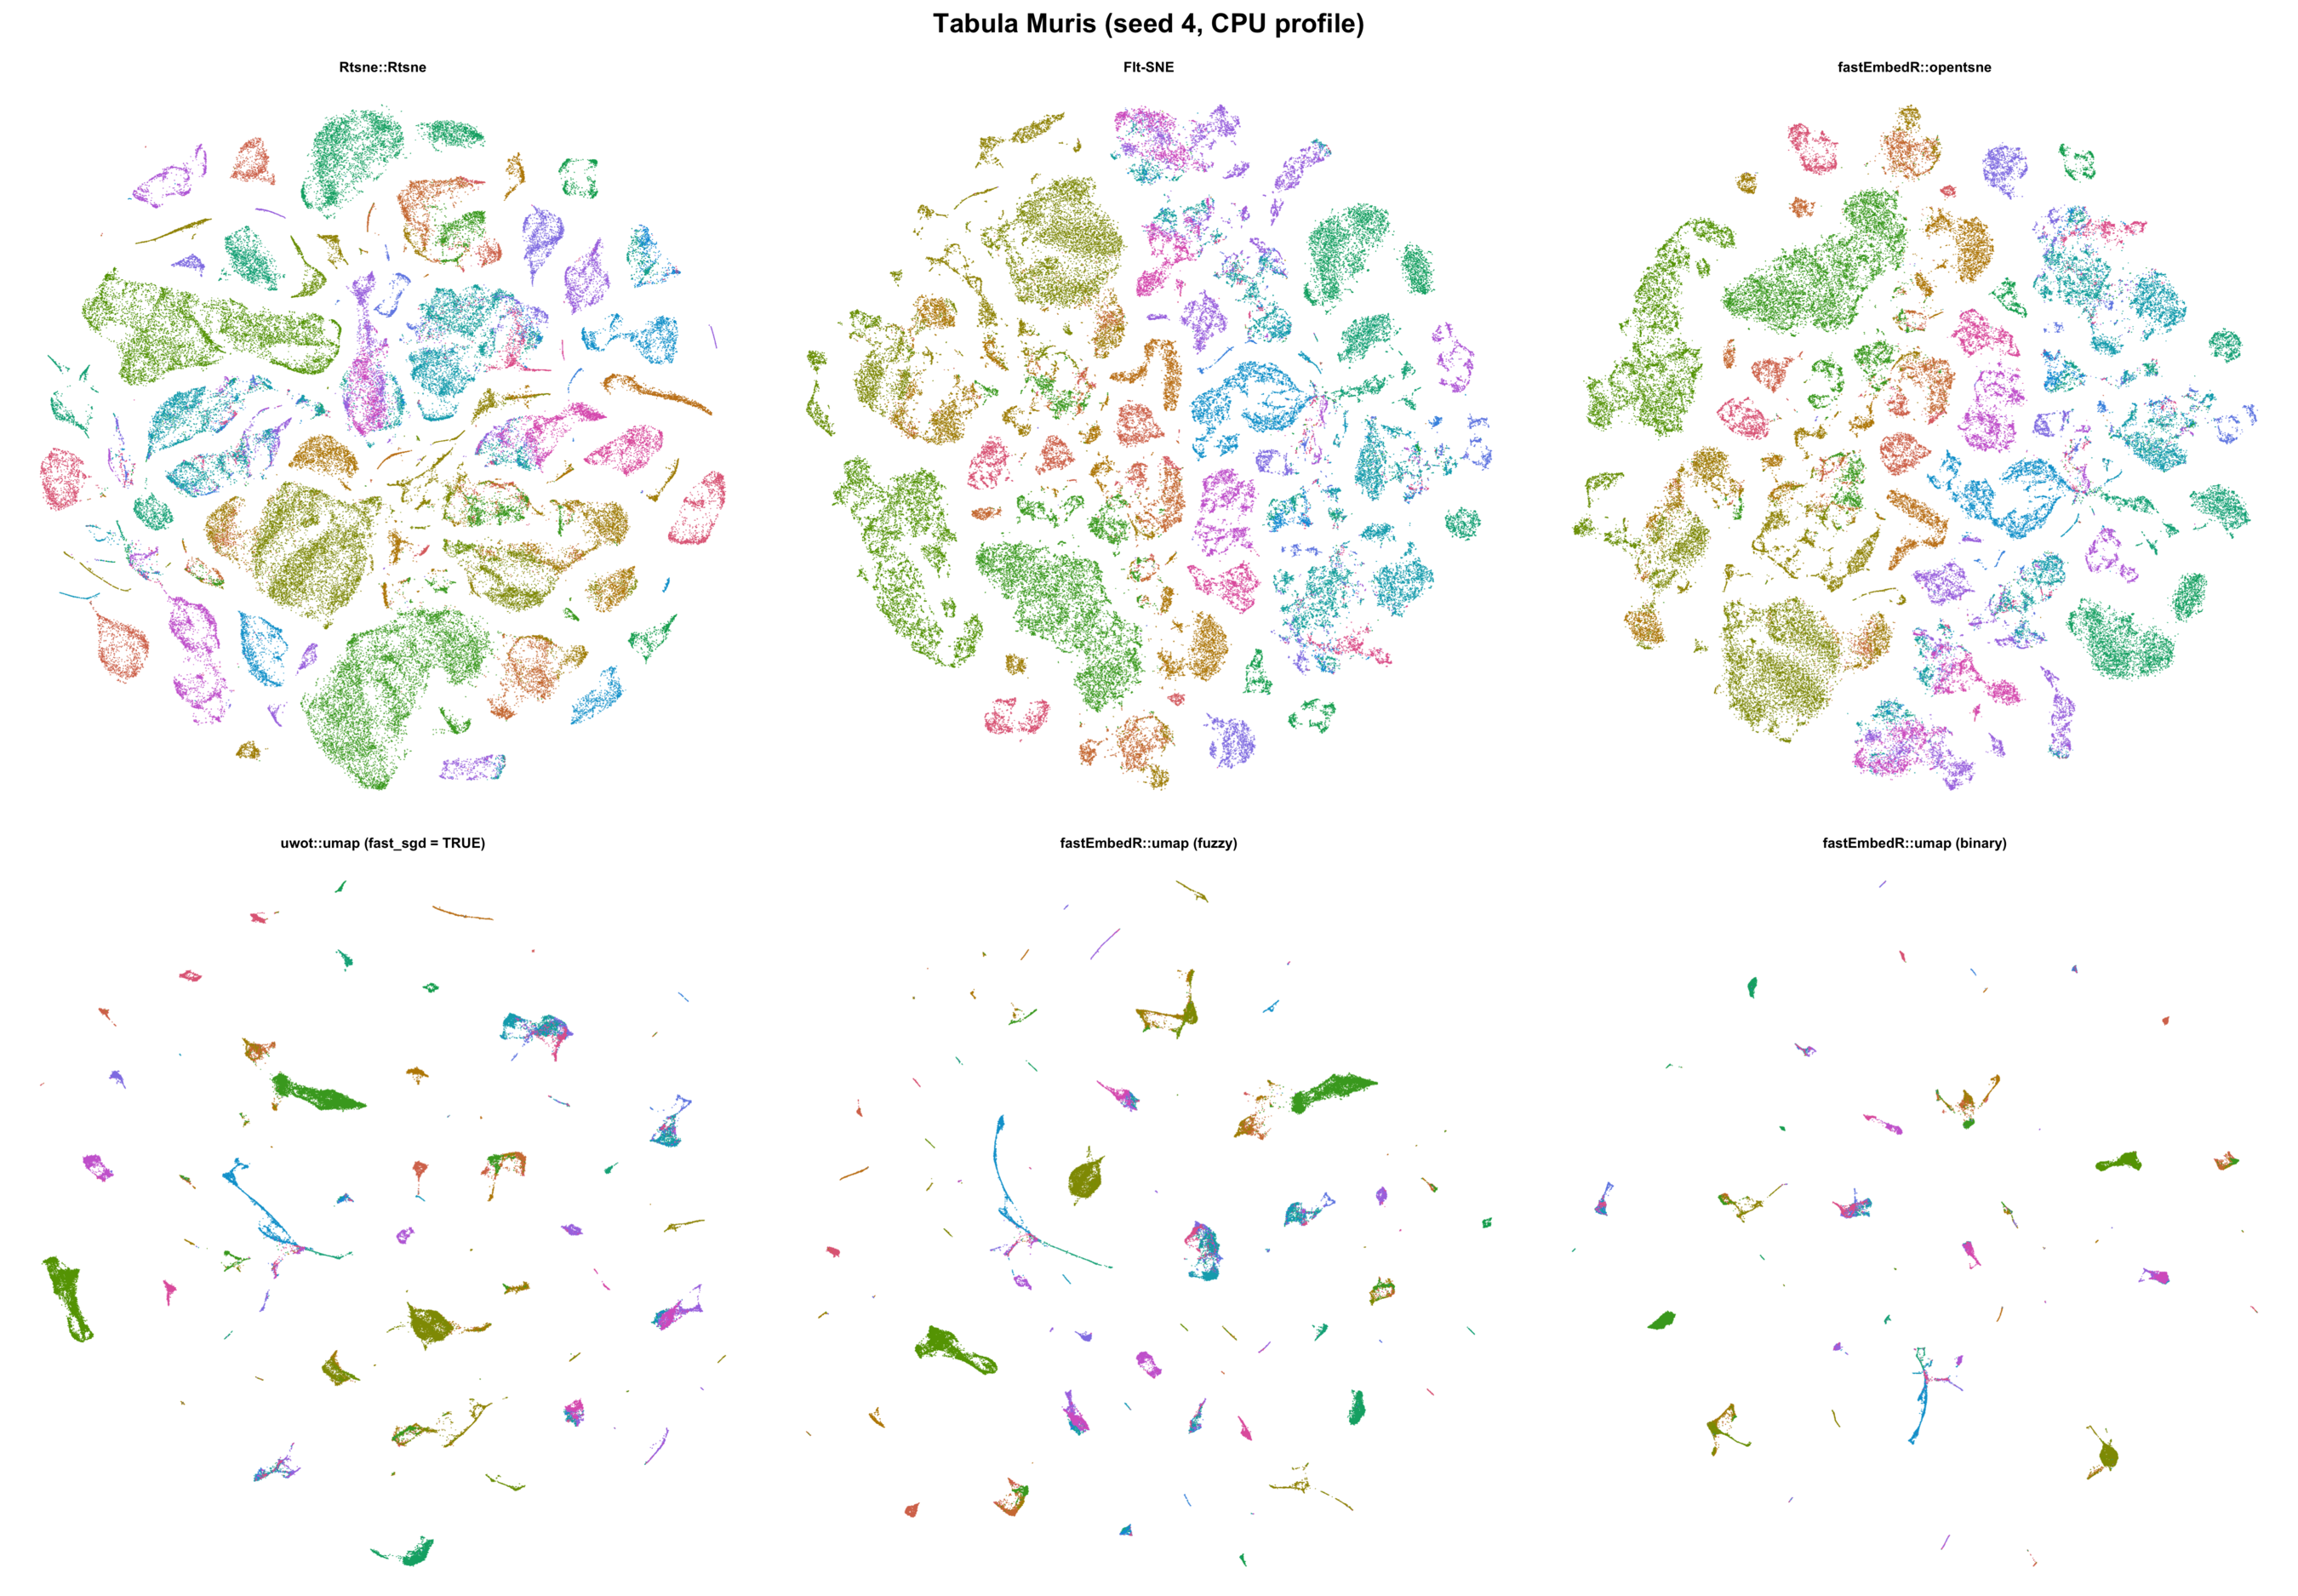
\includegraphics[width=\textwidth]{figures/embedding_comparisons/TabulaMuris_six_methods.png}
\caption{Tabula Muris embeddings for the six selected methods (seed 4; CPU profile unless explicitly marked CUDA). The upper row shows Rtsne, FIt-SNE, and \pkg{} openTSNE; the lower row shows uwot UMAP, \pkg{} fuzzy UMAP, and \pkg{} binary UMAP.}
\label{fig:embeddingtabulamuris}
\end{figure}
\clearpage

\begin{figure}[p]
\centering
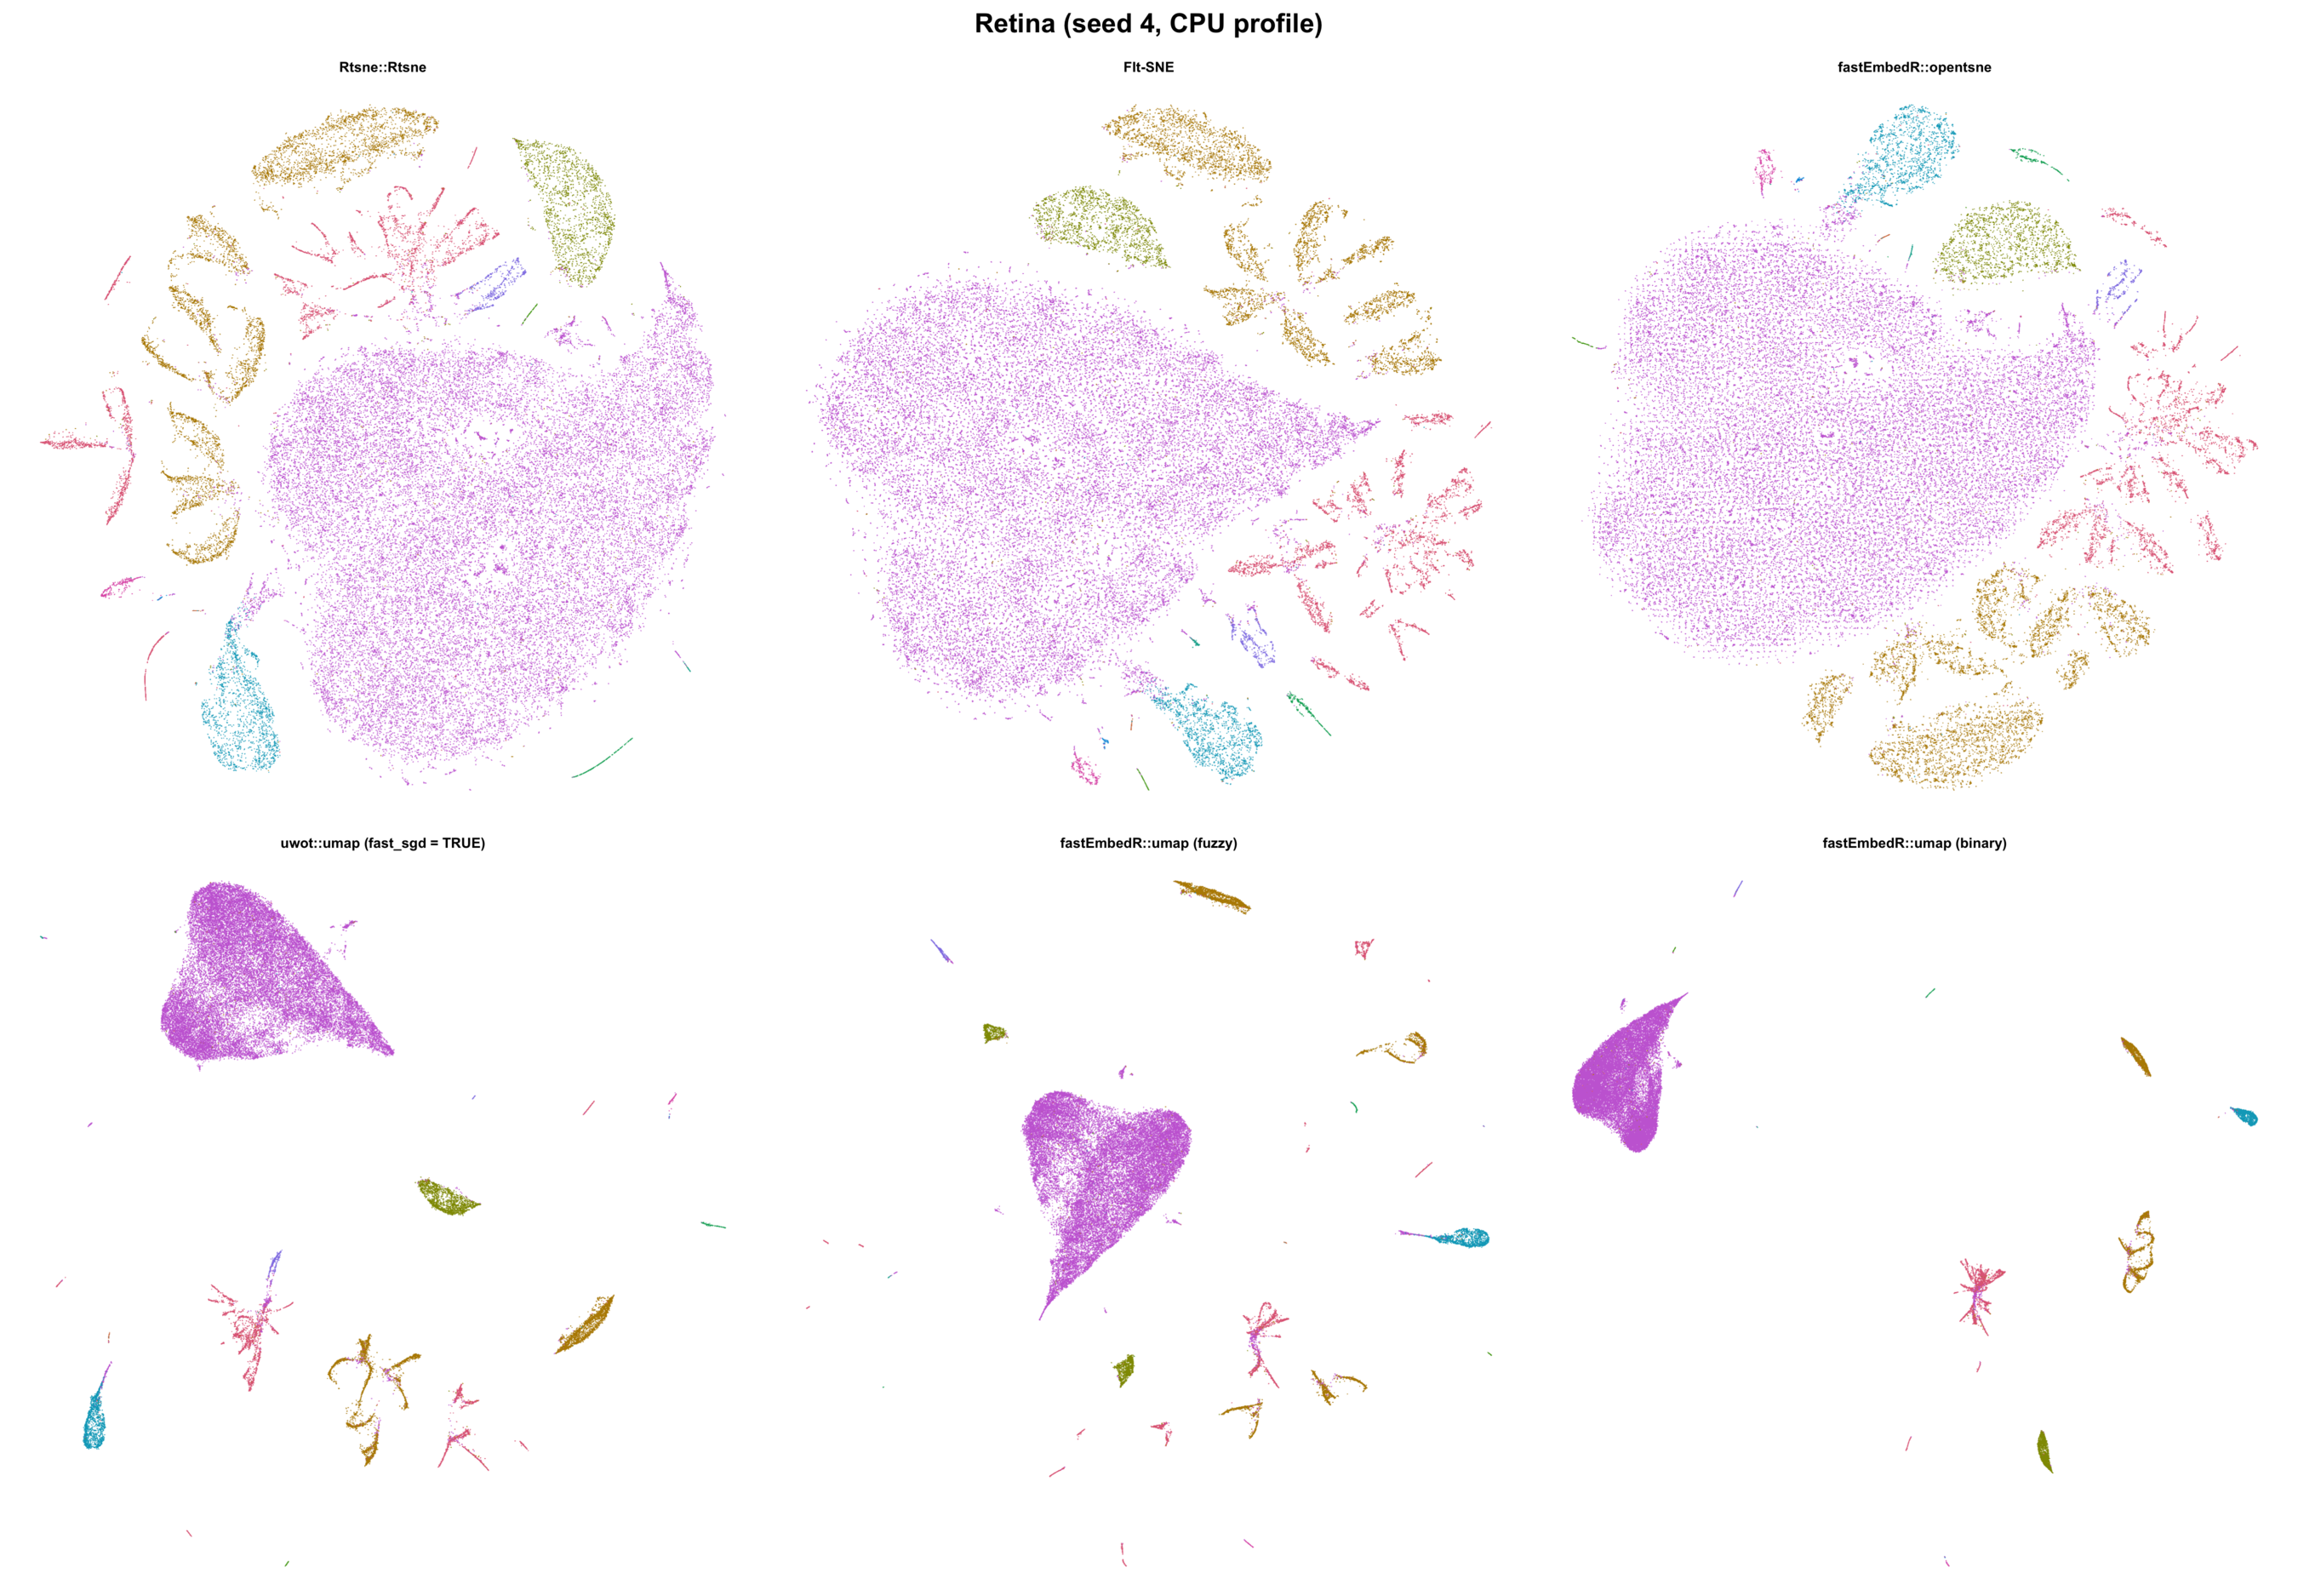
\includegraphics[width=\textwidth]{figures/embedding_comparisons/Macosko2015_retina_six_methods.png}
\caption{Retina embeddings for the six selected methods (seed 4; CPU profile unless explicitly marked CUDA). The upper row shows Rtsne, FIt-SNE, and \pkg{} openTSNE; the lower row shows uwot UMAP, \pkg{} fuzzy UMAP, and \pkg{} binary UMAP.}
\label{fig:embeddingmacosko2015retina}
\end{figure}
\clearpage
